%%%%%%%%%%%%%%%%%%%%%%%%%%%%%%%%%%%%%%%%%%%%%%%%%%%%%%%%%%%%%%%%%%%%%%%%%%
%%
%%	Author Submission Template for Transportation Science (TRSC)
%%	INFORMS, <informs@informs.org>
%%	Ver. 2.00, May 6, 2025 by Matthew Walls
%%
%%%%%%%%%%%%%%%%%%%%%%%%%%%%%%%%%%%%%%%%%%%%%%%%%%%%%%%%%%%%%%%%%%%%%%%%%%
%
% Use dblanonrev for Double Anonymous Review submission
% Use sglanonrev for Single Anonymous Review submission
% For example, submission to Operations Research, OPRE will have
% \documentclass[opre,dblanonrev]{informs4}
%
\documentclass[trsc,dblanonrev]{informs4}
% \documentclass[trsc,sglanonrev]{informs4}
\usepackage{eqndefns-left} % For checking the display equation width and equation environment definitions %
\RequirePackage{tgtermes}
\RequirePackage{newtxtext}
\RequirePackage{newtxmath}
\RequirePackage{bm}
\RequirePackage{endnotes}
\usepackage{changepage} % for adjustwidth
 
\usepackage{amsmath} % for adjustwidth

\usepackage{xcolor}
% Define the custom command
\newcommand{\red}[1]{{\textcolor{red}{#1}}}
%\OneAndAHalfSpacedXI
\OneAndAHalfSpacedXII % Current default line spacing
%%\DoubleSpacedXI
%%\DoubleSpacedXII

% Optional LaTeX Packages
\usepackage{algorithm}
\usepackage{algpseudocode}
\usepackage{tikz}
% Private macros here (check that there is no clash with the style)

% Natbib setup for author-number style
\usepackage{natbib}
 \bibpunct[, ]{(}{)}{,}{a}{}{,}%
 \def\bibfont{\small}%
 \def\bibsep{\smallskipamount}%
 \def\bibhang{24pt}%
 \def\newblock{\ }%
 \def\BIBand{and}%

%% Setup of the equation numbering system. Outcomment only one.
%% Preferred default is the first option.
\EquationsNumberedThrough    % Default: (1), (2), ...
%\EquationsNumberedBySection % (1.1), (1.2), ...

%% Setup of theorem styles. Outcomment only one.
%% Preferred default is the first option.
\TheoremsNumberedThrough     % Preferred (Theorem 1, Lemma 1, Theorem 2)
%\TheoremsNumberedByChapter  % (Theorem 1.1, Lema 1.1, Theorem 1.2)
\ECRepeatTheorems  %  

% For new submissions, leave this number blank.
% For revisions, input the manuscript number assigned by the on-line
% system along with a suffix ".Rx" where x is the revision number.
\MANUSCRIPTNO{TRSC-0001-2024.00}

%%%%%%%%%%%%%%%%
\begin{document}
%%%%%%%%%%%%%%%%

% Outcomment only when entries are known. Otherwise leave as is and
%   default values will be used.
%\setcounter{page}{1}
%\VOLUME{00}%
%\NO{0}%
%\MONTH{Xxxxx}% (month or a similar seasonal id)
%\YEAR{0000}% e.g., 2005
%\FIRSTPAGE{000}%
%\LASTPAGE{000}%
%\SHORTYEAR{00}% shortened year (two-digit)
%\ISSUE{0000} %
%\LONGFIRSTPAGE{0001} %
%\DOI{10.1287/xxxx.0000.0000}%

% Author's names for the running heads
% Sample depending on the number of authors;
% \RUNAUTHOR{Jones}
% \RUNAUTHOR{Jones and Wilson}
% \RUNAUTHOR{Jones, Miller, and Wilson}
% \RUNAUTHOR{Jones et al.} % for four or more authors
% Enter authors following the given pattern:
%\RUNAUTHOR{}
\RUNAUTHOR{Smith and Johnson}

% Title or shortened title suitable for running heads. Sample:
% \RUNTITLE{Predictive Maintenance in Manufacturing}
% Enter the (shortened) title:
\RUNTITLE{}

% Full title. Sample:
% \TITLE{Optimal Resource Allocation in Humanitarian Logistics: A Stochastic Programming Approach}
% Enter the full title:
\TITLE{Synchronising Charging and Break Decisions in the Electric Vehicle Truck Driver Scheduling Problem}

% Block of authors and their affiliations starts here:
% NOTE: Authors with same affiliation, if the order of authors allows,
%   should be entered in ONE field, separated by a comma.
%   \EMAIL field can be repeated if more than one author
\ARTICLEAUTHORS{%
%\AUTHOR{John Doe,\textsuperscript{a} Jane Smith,\textsuperscript{b}}
%\AFF{\textsuperscript{a}Department of Industrial Engineering, University of XYZ, \EMAIL{john.doe@xyz.edu; \textsuperscript{b}Department of Computer Science, University of ABC, \EMAIL{jane.smith@abc.edu}} 
\AUTHOR{}
\AFF{Department of , \EMAIL{}}

\AUTHOR{}
\AFF{Department of , \EMAIL{}}
% Enter all authors
} % end of the block

\ABSTRACT{%
% Enter your abstract
% Please consider using the Structured Abstract as outlined below. This is recommended but not required.
% \textbf{Problem definition:} What is your research problem?
% \textbf{Methodology/results:} What is the research method and the key findings?
% \textbf{Implications:} How can academics / practitioners / policy makers benefit from your paper?
Recent advances in battery technology and fast charging are extending the feasible driving range of battery-electric trucks and enabling their use in long-haul freight transport. In this setting, vehicle operations are tightly constrained by Hours-of-Service regulations that impose mandatory breaks and daily rest periods on drivers. Since recharging is time-consuming and unavoidable on long routes, charging decisions and driver schedules become strongly interdependent. Efficient operation therefore requires synchronizing charging activities with legally mandated interruptions in driving in order to limit increases in route duration. This paper studies the synchronization of charging, breaks, and daily rests for battery-electric trucks operating on fixed long-haul routes spanning multiple days. We introduce a multi-day electric truck driver scheduling problem in which charging decisions are jointly optimized with compliance to Hours-of-Service regulations, with the objective of minimizing total route duration. Methodologically, we extend the labeling-based driver scheduling framework of \textcolor{red}{Goel and Irnich} to incorporate battery charging dynamics, resulting in a resource-constrained shortest path formulation that captures the intertemporal interaction between driving limits, rest structure, and energy constraints. We develop an exact labeling algorithm with tailored resource extension functions and dominance rules that solves the problem to optimality without time discretization. Using a set of benchmark instances constructed from interviews and data collection with long-distance trucking companies operating in Norway and Northern Europe, we conduct a computational analysis of long-haul electric truck schedules. \textcolor{red}{[RESULTS PLACEHOLDER: summarize main numerical findings on route duration, synchronization effects, and structural insights once available.]}
}%

%\FUNDING{This research was supported by [grant number, funding agency].}

%Supplemental Material:
%Data Ethics & Reproducibility Note:

% Sample
%\KEYWORDS{Stochastic programming, Decision support,Uncertainty, Disaster response, Optimization}

% Fill in data. If unknown, outcomment the field
\KEYWORDS{Hours of Service Regulation, Electric Vehicle Routing, Truck Driver Scheduling Problem, Labeling Algorithm, Constrained Shortest Path, Route Synchronization.} 
%\HISTORY{Received: Month DD, YYYY; Accepted: Month DD, YYYY; Published Online: Month DD, YYYY}

\maketitle
%%%%%%%%%%%%%%%%%%%%%%%%%%%%%%%%%%%%%%%%%%%%%%%%%%%%%%%%%%%%%%%%%%%%%%

% Text of your paper here

\section{Introduction}
\label{sec:Intro}

    %quick intro to the problem
    The electrification of road freight transport has progressed rapidly over the last decade. Battery-electric trucks are now being adopted in urban distribution and regional logistics, where vehicles can typically recharge at depots or terminals during predictable off-duty periods (\red{add ref}). Recent improvements in battery capacity and fast-charging technology are extending feasible driving ranges and making longer operations increasingly realistic. Commercial offerings and public information suggest that heavy-duty battery-electric trucks are commonly marketed with single-charge ranges on the order of roughly 300 km, with emerging long-haul models targeting around 500 km under typical operating conditions (\red{add refs Volvo trucks, Mercedes Benz ... etc}). However, long-haul trucking is a low margin business (\red{add ref}) where schedules are tight and time losses translate directly into cost. If charging is treated as an additional stop that “adds time,” long-distance electrification quickly becomes unattractive. This makes smart planning essential: as much charging as possible must be synchronized with time that the driver is legally required to be off-duty anyway.

    %bit more background on HoS truck driver scheduling + charging
    A defining feature of long-haul trucking is that operations are constrained not only by travel and customer time windows, but also by Hours-of-Service (HoS) rules. Under EU regulation, drivers must take mandatory breaks (e.g., a 45-minute break after prolonged driving, potentially split into 15+30 minutes) and mandatory daily rest periods (overnight rests that reset driving/working limits) (\red{add refs -> Drexl, Goel,  Irnich,....?}). For diesel trucks, refueling times are usually short and flexible, so HoS scheduling and energy supply can often be handled separately (\red{add ref}, typically assumed in these papers) . For battery-electric trucks, recharging is time-consuming and location-dependent, and it becomes unavoidable on long routes. As a result, charging and HoS compliance become tightly coupled, especially when route feasibility depends on whether charging can be performed during legally required interruptions in driving.

    %synchronization motivation
    This interdependence gives rise to a critical operational challenge: charging activities must be coordinated with mandatory driver breaks and rests to avoid excessive idle time and loss of productivity. If a driver is required to interrupt driving activity, such interruptions constitute natural opportunities for vehicle charging. When charging activities are systematically aligned with mandated breaks and rest periods, long-haul electric truck operations can remain time-feasible. In contrast, when charging and rest requirements are planned independently, these activities accumulate as separate interruptions, leading to increased route duration and, in extreme cases, to operational infeasibility.

    %relevant literature + gap
    Despite its practical relevance, the joint scheduling of charging and driver interruptions remains underdeveloped for multi-day long-haul operations. The electric vehicle routing and charging literature has largely focused on distribution-style settings and single-day horizons, where synchronization effects are limited and daily rest do not occur (\red{refs}). In parallel, the truck driver scheduling literature provides sophisticated models and algorithms for HoS compliance, but typically assumes conventional vehicles with negligible refueling times (\red{refs}). Only a small number of studies explicitly consider charge–break synchronization, most notably \red{Schiffer et al. (2017)}, and more recently \red{Brockmann and Guajardo (2025)}. However, these contributions are confined to operational regimes closer to regional or single-shift planning and do not address the setting where overnight rests repeat and shape feasibility across multiple driving days. In long-haul trucking, this is exactly where synchronization becomes most important.

    %what do we do
    We therefore study the synchronization of charging, breaks, and daily rests for battery-electric trucks operating on fixed long-haul routes that span multiple days. This setting reflects many real long-distance freight operations where routes and stop sequences are largely predetermined by contracts, infrastructure, and corridor structure, and the dominant planning task is to construct a legally compliant and time-feasible schedule along that route. Given a fixed sequence of customer locations with time windows, we decide when and where to initiate breaks and daily rests, when and where to charge, and how these activities should overlap to minimize total route duration while respecting both HoS and battery feasibility.

    Methodologically, we formulate the problem as a shortest path problem with resource constraints that captures the interdependence between HoS counters and battery state along the route (\red{refs, mention we build on Goel, how do we extend?}). We solve the problem exactly using a labeling algorithm with tailored resource extension functions and dominance rules, enabling synchronized scheduling decisions without time discretization. This yields optimal multi-day schedules under combined regulatory and energy constraints.

    %contributions
    The contributions of this paper are fourfold. First, we introduce a \textbf{multi-day electric truck driver scheduling problem} that explicitly integrates charging decisions with both mandatory breaks and daily rest periods, a setting that has not been addressed in existing %synchronization 
    studies. Second, \textbf{we extend the labeling-based driver scheduling framework} of \red{Goel and Irnich (2017)} to incorporate battery charging dynamics and develop an exact labeling algorithm with tailored resource extension functions and dominance rules, enabling joint optimization of Hours-of-Service compliance and charging decisions without time discretization.
    Third, we \textbf{define and document a set of open-source benchmark instances} for long-haul electric truck scheduling, constructed from interviews and data collection with long-distance trucking companies operating in Norway and Northern Europe.
    Fourth, we provide a \textbf{systematic computational analysis of long-haul electric truck schedules} that quantifies when charging–rest synchronization becomes binding, identifies the structural drivers of infeasibility, and characterizes how route length and rest structure shape optimal charging patterns.

    By extending established driver scheduling methods to account for battery charging, this work clarifies how charging–rest synchronization shapes route duration in long-haul electric trucking and provides a rigorous foundation for the exact analysis of such operations.



\section{Literature Review}
\label{Literature Review}

The electrification of long-haul freight transport in the European Union (EU) introduces novel challenges for logistics planning. Two operationally critical and interdependent factors arise in this context: the need to comply with HoS regulations imposed on drivers, and the effective scheduling of battery charging operations for BETs. These challenges are traditionally addressed within the frameworks of the TDSP and the EVRP, respectively. The TDSP focuses on regulatory compliance regarding driving, rest, and break times \citep{goel2010truck, goel2017exact}, while the EVRP accounts for battery constraints, recharging times, and the positioning of charging stations \citep{desaulniers2016exact, schneider2014electric}. However, a joint treatment of these dimensions—especially in the case of long-haul, fixed-route operations with strict time windows—remains relatively unexplored \citep{schiffer2017impact, schneider2023novel}. This literature review surveys the relevant foundations of the VRP, EVRP, and TDSP, with particular emphasis on approaches that integrate these models. Special attention is given to dynamic programming and labeling algorithms, which are widely used to solve SPPRC, a central formulation in many exact approaches for both TDSP and EVRP \citep{vidal2020concise}.

\subsection{Vehicle Routing Problems and Electric Extensions}

The Vehicle Routing Problem (VRP), first introduced by \citet{dantzig1959truck}, generalizes the classical Traveling Salesman Problem (TSP) to a setting involving multiple vehicles and customer demands. The VRP has since become a key problem in operations research due to its theoretical richness and broad applicability. In its classical form, the VRP aims to determine cost-minimizing routes for a fleet of vehicles serving a set of customers under constraints such as vehicle capacity and route feasibility \citep{jiang2025multi}. The EVRP extends the VRP by incorporating the energy constraints of battery electric vehicles (BEVs). These vehicles must periodically recharge at designated CSs, adding complexity to route planning. The EVRP introduces additional decision variables to track energy consumption, battery state-of-charge (SoC), and recharging operations. Structurally, the problem resembles the VRP with intermediate stops, since CSs may need to be inserted between customer visits to preserve feasibility \citep{schneider2014electric}.

Key modeling choices in EVRP include the placement and distribution of CSs, whether fixed or dynamically inserted into customer sequences \citep{ lam2022branch}, the decision of how much to recharge at each stop, and how energy consumption is modeled. Early EVRP variants assumed constant consumption and fixed or linear recharging times \citep{conrad2011recharging}. More recent studies introduced nonlinear and piecewise-linear charging functions that better reflect realistic charging curves, including the concave current-voltage dynamics of lithium-ion batteries \citep{montoya2017electric}. Additionally, energy tracking has evolved from node-based SoC models to more refined arc-based models that capture energy use and recharging across travel segments \citep{froger2019improved}. These models often include time windows for customer service, as well as vehicle-specific parameters such as battery size and energy efficiency \citep{keskin2019electric, lam2022branch}.

To solve the EVRP, exact methods such as mixed-integer programming (MIP), column generation, and labeling-based algorithms have been proposed. \citet{desaulniers2016exact} present a branch-and-price-and-cut method tailored for several EVRP variants, leveraging strong dominance rules and customized resource extension functions (REFs). In parallel, metaheuristic approaches such as Adaptive Large Neighborhood Search (ALNS) and hybrid heuristics have been applied to solve larger instances with complex charging behaviors \citet{rodriguez2024new}. These algorithmic foundations enable extensions to more realistic EVRP variants, such as those incorporating driver scheduling constraints—a direction explored in this work.

\subsection{Truck Driver Scheduling and Hours of Service Regulations}

The TDSP focuses on generating feasible work schedules for drivers under regulatory HoS constraints. These regulations govern permissible driving time, mandatory breaks, daily and weekly rest periods, and are enforced to promote road safety and labor compliance. The earliest formalization, the Trip Scheduling Problem by \citet{archetti2009trip}, addressed U.S. HoS rules, but earlier works such as \citet{savelsbergh1998drive} already considered breaks in pickup-and-delivery problems.

European HoS regulations are more intricate than those in the U.S., allowing for flexible rest periods, split rests, and stricter weekly limits \citep{goel2009vehicle, drexl2010labelling}. These complexities led to the widespread adoption of dynamic programming approaches, often cast as SPPRC. In these models, resources such as cumulative driving time, rest status, and working hours are encoded into a multi-dimensional state vector propagated through a network using label extension functions.

Key contributions to exact solution methods include the Breadth-First Search labeling algorithm of \citet{goel2010truck}, which introduces pseudo-feasibility and dominance rules to reduce computational burden. \citet{goel2017exact} formalize the Vehicle Routing and Truck Driver Scheduling Problem (VRTDSP) using a branch-and-price framework, where the pricing subproblem becomes an SPPRC with up to nine interacting resources. Label-setting subproblems in this context require strong dominance and tailored extension functions.

Integration of TDSP into routing problems (VRP, VRPTW) has seen diverse modeling strategies. \citet{drexl2010labelling} propose a comprehensive SPPRC framework for EU-compliant Vehicle Routing with Time Windows (VRPTW). \citet{goel2012efficient} account for highway infrastructure limitations by prohibiting stops at arbitrary locations, enhancing realism. Meanwhile, \citet{tilk2020bidirectional} introduce a bidirectional labeling method, where forward and backward labels are joined, enabling more efficient path exploration.

Beyond regulatory compliance, real-world deployment of TDSP models has addressed constraints such as parking availability, long-haul rest infrastructure, and reduced rest allowances. These formulations form a critical foundation for extensions to electric truck operations, where synchronization with recharging activities becomes essential.


\subsection{Joint Optimization of Routing, Charging, and Driver Scheduling}

The EVTDSP represents the integration of two complex optimization domains: electric vehicle routing and regulatory-compliant truck driver scheduling. It requires synchronizing battery charging operations with driver breaks and rest periods, all while respecting service time windows and vehicle range limitations. This integration introduces non-trivial trade-offs between energy and labor constraints, especially in long-haul, fixed-route operations governed by EU HoS regulations.

The most notable contribution toward this integrated problem is the work by \citet{schiffer2017impact}, who propose a mid-haul EVRP with synchronized driver breaks and vehicle recharging. Their model allows breaks to occur at charging stations, customer locations, or dedicated rest stops, and assumes linear charging times proportional to energy demand. Although breaks and charging can be performed simultaneously, the model excludes rest periods and focuses solely on single-shift operations. For larger instances, a modified Adaptive Large Neighborhood Search (ALNS) metaheuristic is employed \citep{schiffer2017solution}, as exact methods struggle with the added complexity of HoS compliance.

A complementary study by \citet{schneider2023novel} explores operational strategies for battery electric vehicles under EU HoS using the emerging Megawatt Charging System (MCS) standard. While the study does not solve a routing problem directly, it evaluates alternative scheduling scenarios—such as single 45-minute breaks or split breaks—under varying battery capacities and consumption levels. The results underscore the need to co-design vehicle range, charging infrastructure, and break timing to ensure regulation-compliant operations.

Existing EVRP formulations such as \citet{desaulniers2016exact} support partial and multiple recharges and use advanced SPPRC labeling algorithms with resource extension functions. However, these models assume fixed routes and battery-only constraints, omitting any consideration of driver HoS. Integrating both types of constraints requires extending the SPPRC framework to include driver state variables such as accumulated driving time and rest history.

To the best of our knowledge, there is currently no published solution method or labeling algorithm that simultaneously schedules breaks, rest periods, and the recharging of electric vehicles—specifically addressing both where and how much to recharge—within a unified framework. This is particularly relevant for multi-shift or multi-day scenarios with open-ended routes. This appears to be an important gap in the literature. In this work, we aim to address this gap by developing a SPPRC-based labeling algorithm tailored to the EVTDSP, capable of producing feasible and synchronized schedules that satisfy both energy and regulatory constraints.


\subsection{Labeling Algorithms and Dynamic Programming}

Labeling algorithms and dynamic programming (DP) are central to solving the Shortest Path Problem with Resource Constraints (SPPRC), a general framework used in both the Truck Driver Scheduling Problem (TDSP) and the Electric Vehicle Routing Problem (EVRP). This framework is particularly well-suited to the Electric Vehicle Truck Driver Scheduling Problem (EVTDSP), where multiple interdependent constraints—such as driving time, rest rules, and battery energy—must be tracked and updated over time.

Dynamic programming decomposes complex scheduling problems into sequential decision stages. At each stage, a state vector of resource values (e.g., time, energy, accumulated driving) is updated through resource extension functions (REFs), and feasible paths are constructed by combining resource-consistent transitions. The SPPRC formulation thus provides a natural structure for encoding legal and physical constraints in EVTDSP.

Labeling algorithms operationalize this structure by defining a label as a tuple of resource values and a partial path. In the EVTDSP context, labels typically track time, battery state-of-charge, driving time since the last break, elapsed working time, rest history, and required recharge duration \citep{goel2017exact}. As labels are extended along arcs in the network, feasibility checks ensure compliance with HoS rules and battery constraints, while dominance rules discard suboptimal labels—usually via Pareto dominance or problem-specific criteria \citep{desaulniers2016exact}.

Several types of labeling strategies have been proposed. Forward labeling is conceptually simple but can generate redundant paths. Backward labeling addresses some of this inefficiency but is harder to combine with real-time constraints. Bidirectional labeling merges the strengths of both, significantly reducing runtime by connecting partial paths from opposite directions. \citet{tilk2020bidirectional} develop a bidirectional method tailored to EU and US HoS regulations, which requires asymmetric REFs and a custom merging strategy.

Despite their flexibility, labeling algorithms suffer from label explosion, especially in high-dimensional problems like the EVTDSP. This necessitates strong pruning techniques and carefully designed REFs to balance completeness and computational efficiency. Nevertheless, the SPPRC labeling paradigm remains the most effective exact approach for solving large-scale, regulation-constrained scheduling problems and forms the algorithmic foundation for the method proposed in this work.


\subsection{Positioning of the Current Work}

While the EVRP and the TDSP have both received substantial attention in the literature, their integration remains underexplored—particularly for realistic, long-haul, multi-shift operations. The only study that explicitly combines TDSP with EVRP is \citet{schiffer2017impact}, which introduces synchronized driver breaks and recharging events. However, that model is limited to daily operations, excludes rest periods, and assumes linear recharging without addressing longer planning horizons or multi-day shifts.

This work addresses that gap by introducing the EVTDSP, formulated on fixed customer routes with time windows. The model fully respects EU HoS regulations, including both mandatory breaks and daily rest periods, while supporting open-ended schedules where vehicles are not required to return to a depot. Battery Electric Trucks (BETs) recharge at regularly spaced, homogeneous charging stations using a linear top-up strategy. Unlike prior work, this model captures the interaction between labor and energy constraints over extended planning periods.

From a methodological perspective, the approach builds on the SPPRC labeling algorithm structure from \citet{goel2017exact} and incorporates recharging mechanics inspired by \citet{desaulniers2016exact}. It extends these frameworks by developing a novel label structure capable of synchronizing breaks, rests, and charging operations. The algorithm includes strong dominance rules, feasibility checks, and support for both partial and multiple recharges, all embedded in a parameter-free network that captures temporal and energy interactions without artificial discretization.

This contribution advances the field in several ways: (i) by enabling realistic scheduling of BET operations under legal and technical constraints, (ii) by introducing a scalable labeling-based solution method for multi-shift, open-ended electric routing problems, and (iii) by providing a general framework that is implementable in real-world logistics planning systems.

To illustrate how the proposed approach compares to prior literature, Table~\ref{tab:Literature_Review} summarizes the key modeling and algorithmic attributes across relevant works. As shown, ours is the only method that simultaneously addresses driver scheduling, charging station use, linear recharging, multiple shifts, and long-haul applicability within a dynamic programming framework.



\begin{table}
\TABLE
{Comparative overview of related works.\label{tab:Literature_Review}}
{\begin{tabular}{@{}p{7.5cm}p{2.2cm}p{3cm}ccccc@{}}
\hline\up
\textbf{Paper} & \textbf{Objective Function} & \textbf{Solution Method} & \textbf{TDS} & \textbf{CS} & \textbf{LCF} & \textbf{MS} & \textbf{LH} \\
\hline\up
\cite{xue2025routing} & Min Time & DP & Yes & Yes & Yes & Yes & Yes \\
\cite{archetti2009trip} & None & PA & Yes & No & No & Yes & No \\
\cite{barco2017optimal} & Min Cost & DEA & No & Yes & No & No & No \\
\cite{campbell2004efficient} & MCO & Heuristic & Yes & No & No & Yes & No \\
\cite{ceselli2009column} & Min Cost & CG, DP & Yes & No & No & No & No \\
\cite{conrad2011recharging} & MCO & Heuristics & No & No & Yes & No & No \\
\cite{de2022using} & Min Cost & DP, Heuristics & No & No & Yes & Yes & Yes \\
\cite{desaulniers2016exact} & Min Cost & BNPNC & No & Yes & Yes & No & No \\
\cite{drexl2010labelling} & MCO & DP & Yes & No & No & Yes & Yes \\
\cite{dolgui2024scheduling} & Min Distance & Heuristics & No & Yes & No & No & Yes \\
\cite{ferro2020optimal} & Min Cost & MIP & No & Yes & Yes & No & No \\
\cite{froger2019improved} & Min Time & DP, Heuristic & No & Yes & No & No & No \\
\cite{goel2009vehicle} & MCO & Heuristic, LNS & Yes & No & No & Yes & No \\
\cite{goel2010truck} & None & BFS & Yes & No & Yes & Yes & Yes \\
\cite{goel2012canadian} & Min Time & DP & Yes & No & Yes & Yes & Yes \\
\cite{goel2012minimum} & Min Time & DP & Yes & No & Yes & Yes & Yes \\
\cite{goel2017exact} & Min Cost & DP & Yes & No & Yes & Yes & Yes \\
\cite{goel2012efficient} & None & DFBSS & Yes & No & No & Yes & Yes \\
\cite{vidal2020concise} & Min Cost & HGSADC & Yes & Yes & No & Yes & Yes \\
\cite{grandinetti2016pick} & MCO & MIP, WSM & No & Yes & Yes & No & No \\
\cite{keskin2019electric} & MCO & Matheuristic & No & No & No & Yes & No \\
\cite{kocc2018long} & Min Cost & Matheuristics, ALNS & Yes & No & No & Yes & Yes \\
\cite{kok2010dynamic} & MCO & DP, Heuristic & Yes & No & No & Yes & Yes \\
\cite{lam2022branch} & Min Cost & BNCNP & No & Yes & No & No & No \\
\cite{lin2016electric} & Min Cost & MIP & No & Yes & Yes & No & No \\
\cite{mayerle2020long} & Min Cost & LNS & Yes & No & No & Yes & Yes \\
\cite{montoya2017electric} & Min Time & Hybrid Metaheuristic & No & Yes & No & No & No \\
\cite{pelletier2018charge} & Min Cost & MIP & No & No & No & Yes & No \\
\cite{prescott2010european} & Min Cost & LNS, labeling & Yes & No & No & Yes & No \\
\cite{rancourt2013long} & MCO & Tabu Search & Yes & No & No & Yes & Yes \\
\cite{savelsbergh1998drive} & MCO & BNP & Yes & No & No & Yes & No \\
\cite{schiffer2017impact} & Min Cost & MIP, ALNS & Yes & Yes & Yes & No & No \\
\cite{schneider2014electric} & MCO & Hybrid Heuristic & No & Yes & Yes & No & Yes \\
\cite{schneider2023novel} & None & -- & Yes & Yes & No & Yes & Yes \\
\cite{tilk2020bidirectional} & Min Cost & BNCNP, DP & Yes & No & No & Yes & Yes \\
\cite{vital2021scheduling} & Min Cost & DP & Yes & No & Yes & No & No \\
\cite{xu2003solving} & Min Cost & Matheuristics, DP & Yes & No & Yes & No & No \\
Current Study & Min Cost & DP & Yes & Yes & Yes & Yes & Yes \down\\
\hline
\end{tabular}}
{TDS = Truck Driver Scheduling, CS = Charging Stations, LCF = Linear Charging Function, MS = Multiple Shifts, LH = Long-Haul.}
\end{table}
% 




%-------main template 
\section{Problem Description}
\label{PROBLEM DESCRIPTION}

This work addresses the EVTDSP, which arises in long-haul freight operations using BETs. The problem requires constructing a feasible schedule that jointly satisfies driver labor regulations—specifically the HoS rules mandated in the European Union and electric vehicle energy constraints. The objective is to minimize the total time required to complete a fixed customer route, while determining optimal locations and durations for breaks, rest periods, and battery charging.

We consider a single BET operated by one driver, assigned to a fixed and pre-determined sequence of customer locations. The route is assumed to be feasible in terms of travel distance and customer connectivity. Each customer location is associated with a hard time window within which service must begin. These time windows reflect the operational hours of facilities such as warehouses or retail centers and cannot be violated. Service at each customer requires a specified, non-interruptible duration. We assume that the vehicle's cargo load does not affect energy consumption, and all distances and travel times between locations are known in advance.

The BET is equipped with a battery of fixed capacity, measured in kilowatt-hours (kWh), and consumes energy at a constant rate proportional to distance traveled. The vehicle may recharge its battery at CSs located at uniform intervals along the route. All CSs are homogeneous and provide energy at a fixed power level, implying a linear relationship between charging time and energy gained. Charging can be performed in partial increments, and multiple charging stops are permitted throughout the route. However, recharging is not allowed during customer service.

The driver is subject to EU HoS regulations, which define allowable driving and working durations, as well as mandatory break and rest periods. Driving time includes only the operation of the vehicle between locations, while working time encompasses both driving and service time at customers. A break is a short pause typically lasting at least 45 minutes, required after a maximum of 4.5 hours of driving. A daily rest is a longer, uninterrupted period, generally lasting at least 11 hours, and is required after a maximum of 9 hours of driving or 13 hours of total working time. The regulation allows limited flexibility, such as the use of split rests or reduced rest durations under certain conditions.

Breaks and rest periods must not be scheduled during customer service but may be taken at customer locations, at charging stations, or at intermediate points along the route. When breaks or rests occur at a charging station, it is possible for charging and resting activities to overlap, provided neither conflicts with other constraints. Conversely, charging and service activities are mutually exclusive. At each possible stopping location whether it is a customer, a charging station, or a roadside point the model must decide whether to initiate a break or rest, whether to charge the battery, and, if charging is selected, how much energy to add. These decisions are subject to temporal, regulatory, and physical constraints, and collectively determine the total time required to complete the route.

The total route time includes the cumulative driving time between locations, the time spent providing service at each customer, the time allocated to charging, breaks, and rests, and any idle time due to early arrivals at customer locations. Managing these elements requires simultaneously coordinating multiple interdependent factors: the driver's state, the battery's energy level, and customer time windows. The overall objective is to minimize this total route duration by optimally synchronizing the truck driver’s mandatory rest and break periods with battery recharging stops. The structure and constraints of the EVTDSP make it well-suited to a dynamic programming solution based on a shortest path problem with resource constraints (SPPRC), where each path extension updates the state of time, energy, and regulatory compliance. The methodological framework for solving this problem is described in the following section.


\section{Methodology}

The EVTDSP considered in this work addresses the challenge of constructing feasible and efficient schedules for BETs operating under EU HoS regulations. The vehicle follows a fixed, predetermined customer route. In contrast to classical vehicle routing problems (e.g., VRPTW), where travel and service times are sufficient for feasibility validation, the EVTDSP requires explicit modeling of individual driver activities and vehicle energy levels due to regulatory and technological constraints. Under EU HoS regulations, drivers must adhere to a complex set of rules involving cumulative driving time, required breaks, daily rest periods, and maximum working durations. These legal constraints are temporally interdependent and cannot be satisfied by simply adjusting arrival times or inserting passive waiting. Instead, feasible schedules must specify the exact timing and type of each legal activity whether driving, resting, or taking a break. Moreover, these driver states evolve over time and must be tracked in accordance with multiple overlapping limits.

In parallel, BET operations introduce energy-related constraints that interact with the driver's legal requirements. Battery capacities, consumption rates, and limited availability of charging infrastructure necessitate careful planning of when and where to recharge. Charging durations depend on both energy demand and charging power, and these recharging events must often be synchronized with driver rest or break periods to maintain overall route feasibility and minimize delays. Together, these constraints create a high-dimensional, tightly coupled scheduling problem. To solve this challenge, we adopt a labeling-based algorithm operating over a parameter-free network. This approach builds upon the framework proposed by ~\cite{goel2017exact}, which models driver activities using a compact, non-discretized auxiliary network structure and a set of resource extension functions (REFs). In our work, this framework is extended to capture the energy dynamics of electric trucks and their integration with regulatory driver behavior.

\subsection{Parameter-Free Network Representation}\label{sec:ParamFreeNetwork}

To efficiently model the scheduling constraints of the EVTDSP, we build upon the parameter-free network structure proposed by \citet{goel2017exact}. Unlike traditional time-expanded networks, which discretize time and suffer from combinatorial explosion, the parameter-free model represents feasible transitions between locations without discretization. This compact structure enables dynamic programming and dominance-based pruning while preserving regulatory and physical feasibility.

In our setting, the network is defined as \( G = (N, A) \), where \( N \) includes all customer locations and charging stations, and \( A \subseteq N \times N \) represents the set of feasible transitions. Each original arc \( (n, m) \in A \) is replaced by a parameter-free subnetwork \( G''_{nm} = (N''_{nm}, A''_{nm}) \), which compactly encodes all admissible sequences of driving, breaks, rests, and recharging required to travel from node \( n \) to node \( m \). A visualization of such a subnetwork is shown in Figure~\ref{fig:subnetwork_nm}.

\begin{figure}
\FIGURE
{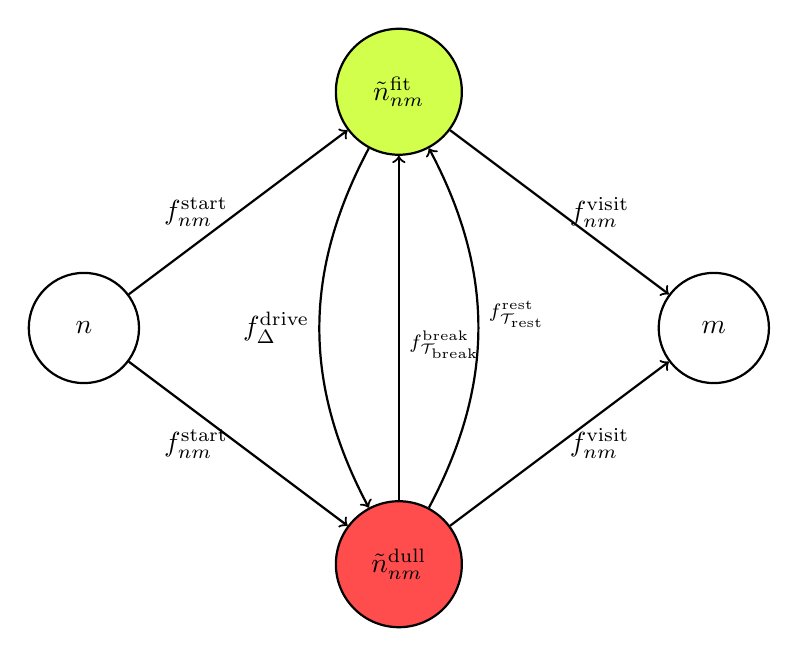
\begin{tikzpicture}[->, thick, auto]
% Node styles
\tikzstyle{main} = [circle, draw=black, minimum size=1.4cm, inner sep=0pt]
\tikzstyle{fit} = [circle, draw=black, fill=lime!70, minimum size=1.6cm, inner sep=0pt]
\tikzstyle{dull} = [circle, draw=black, fill=red!70, minimum size=1.6cm, inner sep=0pt]
% Nodes
\node[main] (n) at (0,0) {$n$};
\node[main] (m) at (8,0) {$m$};
\node[fit] (fit) at (4,3) {$\tilde{n}_{nm}^{\text{fit}}$};
\node[dull] (dull) at (4,-3) {$\tilde{n}_{nm}^{\text{dull}}$};
% Arrows from n to intermediates
\path (n) edge node[left] {$f^{\text{start}}_{nm}$} (fit);
\path (n) edge node[left] {$f^{\text{start}}_{nm}$} (dull);
% Arrows from intermediates to m
\path (fit) edge node[right] {$f^{\text{visit}}_{nm}$} (m);
\path (dull) edge node[right] {$f^{\text{visit}}_{nm}$} (m);
% Curved arrows between intermediates
\path[bend right=28] (dull) edge node[right, yshift=5pt] {\scriptsize $f^{\text{rest}}_{\mathcal{T}_{\text{rest}}}$} (fit);
\path (dull) edge node[right, yshift=-6pt] {\scriptsize $f^{\text{break}}_{\mathcal{T}_{\text{break}}}$} (fit);
\path[bend right=28] (fit) edge node[left] {$f^{\text{drive}}_{\Delta}$} (dull);
\end{tikzpicture}}
{Subnetwork \(G''_{nm}\) of the parameter-free network \(G''\). \label{fig:subnetwork_nm}}
{Text of the notes.}
\end{figure}

Each subnetwork \( G''_{nm} \) consists of three key elements: the origin node \( n \), the destination node \( m \), and two auxiliary intermediate nodes. The first intermediate node, denoted as \( \tilde{n}^{\text{fit}}_{nm} \), represents a state where a new activity can begin, such as starting a driving segment or initiating a charging operation. The second, \( \tilde{n}^{\text{dull}}_{nm} \), captures the continuation or termination of an ongoing activity, for instance completing a break or finishing a rest. These intermediate states allow precise modeling of the allowable transitions between customer nodes without discretizing time, and they serve as anchor points for activity-specific resource extension functions (REFs) that govern the evolution of the driver and vehicle state.

\begin{figure}
\FIGURE
{\resizebox{\textwidth}{!}{%
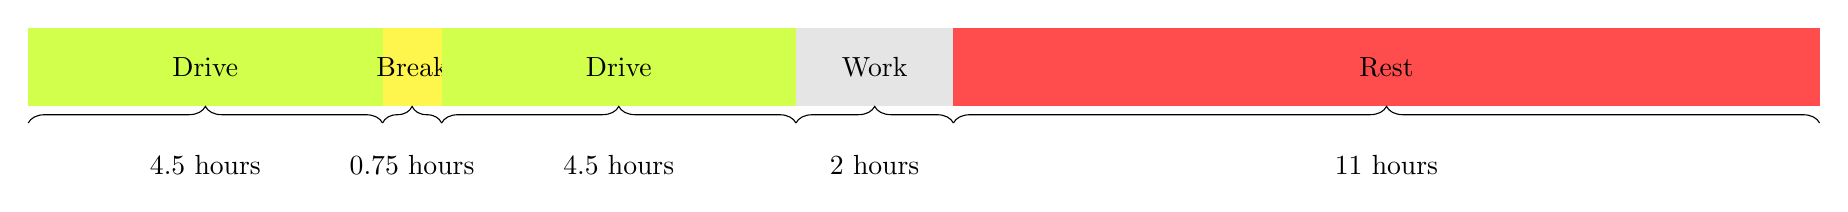
\begin{tikzpicture}
% Time blocks
\def\y{0} % vertical level
\def\h{1} % height of blocks
% Colored rectangles
\fill[fill=lime!70] (0,\y) rectangle (4.5,\y+\h);
\node at (2.25,\y+0.5) {Drive};
\fill[fill=yellow!70] (4.5,\y) rectangle (5.25,\y+\h);
\node at (4.875,\y+0.5) {Break};
\fill[fill=lime!70] (5.25,\y) rectangle (9.75,\y+\h);
\node at (7.5,\y+0.5) {Drive};
\fill[fill=gray!20] (9.75,\y) rectangle (11.75,\y+\h);
\node at (10.75,\y+0.5) {Work};
\fill[fill=red!70] (11.75,\y) rectangle (22.75,\y+\h);
\node at (17.25,\y+0.5) {Rest};
% Brackets and labels
\draw[decorate,decoration={brace,amplitude=6pt},yshift=-6pt] (0,\y) -- (4.5,\y) node[midway,below=8pt] {4.5 hours};
\draw[decorate,decoration={brace,amplitude=6pt},yshift=-6pt] (4.5,\y) -- (5.25,\y) node[midway,below=8pt] {0.75 hours};
\draw[decorate,decoration={brace,amplitude=6pt},yshift=-6pt] (5.25,\y) -- (9.75,\y) node[midway,below=8pt] {4.5 hours};
\draw[decorate,decoration={brace,amplitude=6pt},yshift=-6pt] (9.75,\y) -- (11.75,\y) node[midway,below=8pt] {2 hours};
\draw[decorate,decoration={brace,amplitude=6pt},yshift=-6pt] (11.75,\y) -- (22.75,\y) node[midway,below=8pt] {11 hours};
\end{tikzpicture}
}}
{Example of a schedule of a fully rested driver in accordance with EU HoS regulation. \label{fig:driver_schedule}}
{Text of the notes.}
\end{figure}

The distinction between fit and dull nodes enables an accurate representation of the evolving driver state over time. As a driver progresses along the route, labels transition through these nodes using activity-specific resource extension functions (REFs). These transitions are constrained to ensure that only legally permissible sequences of driving, break, and rest activities are allowed under EU Hours of Service regulations. An example of a valid HoS-compliant schedule is shown in Figure~\ref{fig:driver_schedule}.

The traversal from node \( n \) to node \( m \) in the subnetwork \( G''_{nm} \) depends on the feasibility of the arc \( f^{\text{drive}}_{\Delta} \), which captures the cumulative driving distance and time between \( n \) and \( m \) through REFs. This arc reflects the physical movement between the two nodes, and becomes traversable only when all associated regulatory and physical constraints are satisfied. Once the condition for \( f^{\text{drive}}_{\Delta} \) is satisfied, a label may progress from the intermediate node \( \tilde{n}^{\text{fit}}_{nm} \) to \( \tilde{n}^{\text{dull}}_{nm} \), and subsequently to the destination node \( m \) via \( f^{\text{visit}}_{nm} \). The network structure allows for three logically distinct traversal alternatives between \( n \) and \( m \), each corresponding to a different sequencing of break, rest, and driving activities.

In the first case, a direct drive is performed without any intermediate break or rest:
\begin{align*}
n &\xrightarrow{f^{\text{start}}_{nm}} \tilde{n}^{\text{fit}}_{nm}
\xrightarrow{f^{\text{drive}}_{\Delta}} \tilde{n}^{\text{dull}}_{nm}
\xrightarrow{f^{\text{visit}}_{nm}} m.
\end{align*}

A second possibility arises when the driver needs a post-drive recovery:
\begin{align*}
n &\xrightarrow{f^{\text{start}}_{nm}} \tilde{n}^{\text{fit}}_{nm}
\xrightarrow{f^{\text{drive}}_{\Delta}} \tilde{n}^{\text{dull}}_{nm}
\xrightarrow{f^{\text{break}}_{\mathcal{T}_{\text{break}}}\ \text{or}\ f^{\text{rest}}_{\mathcal{T}_{\text{rest}}}}
\tilde{n}^{\text{fit}}_{nm}
\xrightarrow{f^{\text{visit}}_{nm}} m.
\end{align*}

A third alternative involves pre-drive recovery:
\begin{align*}
n &\xrightarrow{f^{\text{start}}_{nm}} \tilde{n}^{\text{dull}}_{nm}
\xrightarrow{f^{\text{break}}_{\mathcal{T}_{\text{break}}}\ \text{or}\ f^{\text{rest}}_{\mathcal{T}_{\text{rest}}}}
\tilde{n}^{\text{fit}}_{nm}
\xrightarrow{f^{\text{drive}}_{\Delta}} \tilde{n}^{\text{dull}}_{nm}
\xrightarrow{f^{\text{visit}}_{nm}} m.
\end{align*}

To make the parameter-free network compatible with BETs, we must adapt the structure to include charging infrastructure. Specifically, we introduce CS nodes at regular intervals along each arc connecting customer nodes. However, these CS nodes are not mandatory visit points. Instead, their inclusion enables the synchronization of recharging activities with driver breaks and rest periods. The resulting expanded subnetwork is illustrated in Figure~\ref{fig:subnetwork_cs}, which extends the basic form shown earlier in Figure~\ref{fig:subnetwork_nm}.

\begin{figure}
\FIGURE
{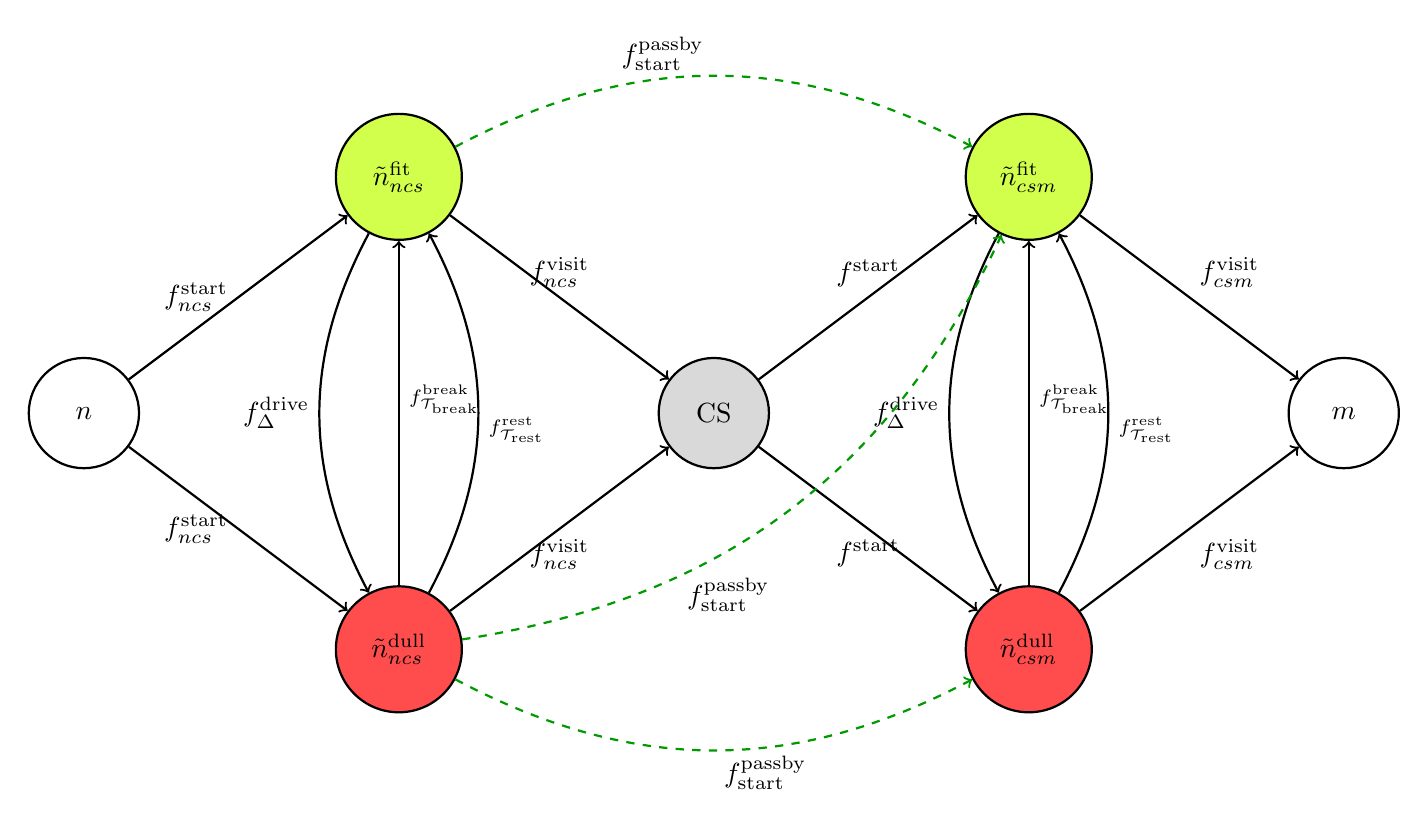
\begin{tikzpicture}[->, thick, auto]
% Node styles
\tikzstyle{main} = [circle, draw=black, minimum size=1.4cm, inner sep=0pt]
\tikzstyle{fit}  = [circle, draw=black, fill=lime!70, minimum size=1.6cm, inner sep=0pt]
\tikzstyle{dull} = [circle, draw=black, fill=red!70, minimum size=1.6cm, inner sep=0pt]
\tikzstyle{cs}   = [circle, draw=black, fill=gray!30, minimum size=1.4cm, inner sep=0pt]
% Nodes
\node[main] (n) at (0,0) {$n$};
\node[fit]  (fitL) at (4, 3) {$\tilde{n}^{\text{fit}}_{ncs}$};
\node[dull] (dullL) at (4, -3) {$\tilde{n}^{\text{dull}}_{ncs}$};
\node[cs]   (cs) at (8, 0) {CS};
\node[fit]  (fitR) at (12, 3) {$\tilde{n}^{\text{fit}}_{csm}$};
\node[dull] (dullR) at (12, -3) {$\tilde{n}^{\text{dull}}_{csm}$};
\node[main] (m) at (16,0) {$m$};
% From n to left states
\path (n) edge node[left] {$f^{\text{start}}_{ncs}$} (fitL);
\path (n) edge node[left] {$f^{\text{start}}_{ncs}$} (dullL);
% Transitions between fit/dull (left side)
\path[bend right=28] (fitL) edge node[left] {$f^{\text{drive}}_{\Delta}$} (dullL);
\path (dullL) edge node[right, yshift=5pt] {\scriptsize $f^{\text{break}}_{\mathcal{T}_{\text{break}}}$} (fitL);
\path[bend right=28] (dullL) edge node[right, yshift=-6pt] {\scriptsize $f^{\text{rest}}_{\mathcal{T}_{\text{rest}}}$} (fitL);
% To CS
\path (fitL) edge node[above] {$f^{\text{visit}}_{ncs}$} (cs);
\path (dullL) edge node[below] {$f^{\text{visit}}_{ncs}$} (cs);
% From CS to right states
\path (cs) edge node[above] {$f^{\text{start}}$} (fitR);
\path (cs) edge node[below] {$f^{\text{start}}$} (dullR);
% Transitions between fit/dull (right side)
\path[bend right=28] (fitR) edge node[left] {$f^{\text{drive}}_{\Delta}$} (dullR);
\path (dullR) edge node[right, yshift=5pt] {\scriptsize $f^{\text{break}}_{\mathcal{T}_{\text{break}}}$} (fitR);
\path[bend right=28] (dullR) edge node[right, yshift=-6pt] {\scriptsize $f^{\text{rest}}_{\mathcal{T}_{\text{rest}}}$} (fitR);
% From right states to m
\path (fitR) edge node[above right] {$f^{\text{visit}}_{csm}$}  (m);
\path (dullR) edge node[below right] {$f^{\text{visit}}_{csm}$} (m);
% Passing-by arcs
\path[->, dashed, thick, green!60!black, bend left=28]
  (fitL) edge node[left, yshift=8pt] {\textcolor{black}{$f^{\text{passby}}_{\text{start}}$}} (fitR);
\path[->, dashed, thick, green!60!black, bend right=28]
  (dullL) edge node[right, xshift=-40pt, yshift=-30pt] {\textcolor{black}{$f^{\text{passby}}_{\text{start}}$}} (fitR);
\path[->, dashed, thick, green!60!black, bend right=28]
  (dullL) edge node[right, yshift=-8pt] {\textcolor{black}{$f^{\text{passby}}_{\text{start}}$}} (dullR);
\end{tikzpicture}}
{Extended subnetwork with a charging station (CS) enabling transitions between fit/dull states across nodes \(n\) and \(m\). \label{fig:subnetwork_cs}}
{Text of the notes.}
\end{figure}

The subnetwork between any two city nodes \( n \) and \( m \) must now include at least one intermediate charging station node. This adjustment makes the structure more flexible, but also introduces new challenges: it must still accommodate all valid transitions between \( n \) and \( m \), including the three previously described alternatives involving breaks, rests, or direct driving. The presence of a CS between \( n \) and \( m \) enables additional opportunities for synchronization, but also requires careful treatment of how and when charging actually occurs. A critical design question arises when the label encounters a CS node but the vehicle does not need to recharge. In this case, the algorithm must support a passing-by mechanism that allows the label to skip the charging operation. To facilitate this, we introduce special arcs, referred to as \( \tilde{n}^{\text{passby}}_{cs} \) arcs, between intermediate nodes located before and after a CS. These arcs allow the label to maintain continuity through the CS without performing a recharge.

In order to traverse a passing-by arc, the same conditions that allow visiting a CS must be satisfied: namely, the arc \( f^{\text{drive}}_{\Delta} \) from \( n \) to the CS must be feasible, ensuring that the required driving time and energy have been accumulated. Furthermore, the label must be able to continue from the CS to \( m \) without violating battery or HoS constraints. Thus, whenever the condition for visiting a CS is satisfied, the condition for passing-by is also satisfied. The REF used to implement passing-by arcs is denoted \( f^{\text{passby}}_{\text{start}} \). It functions similarly to \( f^{\text{start}}_{nm} \), but it skips the charging operation and simply adds the remaining travel time from the CS to the next node. This REF maintains label continuity and ensures that both energy and time are tracked correctly. A complete definition and explanation of all REFs, including \( f^{\text{passby}}_{\text{start}} \), is provided in the next subsection.

Another structural concern is how to connect the intermediate nodes on either side of a CS in the virtual graph. To support all traversal possibilities across a CS, whether charging occurs or not, we must add arcs between specific pairs of intermediate nodes before and after the CS. These arcs are required to ensure that the three possible transitions from \( n \) to the CS and from the CS to \( m \) are fully represented in the network. To achieve this, three specific types of passing arcs are introduced.

First, we connect the ``fit'' node before the CS to the ``fit'' node after the CS:
\begin{align*}
\tilde{n}^{\text{fit}}_{\text{before}} &\xrightarrow{f^{\text{passby}}} \tilde{n}^{\text{fit}}_{\text{after}}
\xrightarrow{f^{\text{drive}}_{\Delta}} \tilde{n}^{\text{dull}}_{\text{after}}
\xrightarrow{f^{\text{visit}}} m,
\end{align*}
or
\begin{align*}
\tilde{n}^{\text{fit}}_{b}
&\xrightarrow{f^{\text{passby}}}
\tilde{n}^{\text{fit}}_{a}
\xrightarrow{f^{\text{drive}}_{\Delta}}
\tilde{n}^{\text{dull}}_{a}
\xrightarrow[
  f^{\text{rest}}_{\mathcal{T}_{\text{rest}}}
]{
  f^{\text{break}}_{\mathcal{T}_{\text{break}}}
}
\tilde{n}^{\text{fit}}_{a}
\xrightarrow{f^{\text{visit}}}
m.
\end{align*}

Second, we connect the ``dull'' node before the CS to the ``dull'' node after the CS:
\begin{align*}
\tilde{n}^{\text{dull}}_{\text{b}} &\xrightarrow{f^{\text{passby}}} \tilde{n}^{\text{dull}}_{\text{a}}
\xrightarrow[
  f^{\text{rest}}_{\mathcal{T}_{\text{rest}}}
]{
  f^{\text{break}}_{\mathcal{T}_{\text{break}}}
}
\tilde{n}^{\text{fit}}_{\text{a}}
\xrightarrow{f^{\text{drive}}_{\Delta}} \tilde{n}^{\text{dull}}_{\text{a}}
\xrightarrow{f^{\text{visit}}} m.
\end{align*}

Finally, we connect the ``dull'' node before the CS to the ``fit'' node after the CS:
\begin{align*}
\tilde{n}^{\text{dull}}_{b}
&\xrightarrow{f^{\text{passby}}}
\tilde{n}^{\text{fit}}_{a}
\xrightarrow{f^{\text{drive}}_{\Delta}}
\tilde{n}^{\text{dull}}_{a}
\xrightarrow{f^{\text{visit}}}
m,
\end{align*}
or
\begin{align*}
\tilde{n}^{\text{dull}}_{b}
&\xrightarrow{f^{\text{passby}}}
\tilde{n}^{\text{fit}}_{a}
\xrightarrow{f^{\text{drive}}_{\Delta}}
\tilde{n}^{\text{dull}}_{a}
\xrightarrow[
  f^{\text{rest}}_{\mathcal{T}_{\text{rest}}}
]{
  f^{\text{break}}_{\mathcal{T}_{\text{break}}}
}
\tilde{n}^{\text{fit}}_{a}
\xrightarrow{f^{\text{visit}}}
m.
\end{align*}


The combination of these arcs ensures that all feasible trajectories through CS nodes—including optional recharging, synchronized breaks, or simply passing by—can be modeled within the parameter-free network. A complete enumeration of possible cases is illustrated in Table~\ref{tab:cs_cases}, and visualized through the extended subnetwork in Figure~\ref{fig:subnetwork_cs}.

\begin{table}
\TABLE
{Feasible path combinations for transitions between \(n \rightarrow \text{CS}\) and \(\text{CS} \rightarrow m\) in the expanded parameter-free network.\label{tab:cs_cases}}
{\begin{tabular}{@{}p{6.5cm}p{8cm}@{}}
\hline\up
\textbf{Traversal from \(n\) to CS} & \textbf{Traversal from CS to \(m\)} \\
\hline\up
$\tilde{n}^{\text{dull}} \xrightarrow{f^{\text{drive}}} \tilde{n}^{\text{fit}} \xrightarrow{f^{\text{break}} \text{ or } f^{\text{rest}}} \tilde{n}^{\text{dull}}$
&
\begin{tabular}[t]{@{}l@{}}
$\tilde{n}^{\text{fit}} \xrightarrow{f^{\text{drive}}} \tilde{n}^{\text{dull}} \xrightarrow{f^{\text{visit}}} m$ \\
$\tilde{n}^{\text{fit}} \xrightarrow{f^{\text{drive}}} \tilde{n}^{\text{dull}} \xrightarrow{f^{\text{break}} \text{ or } f^{\text{rest}}} \tilde{n}^{\text{fit}} \xrightarrow{f^{\text{visit}}} m$ \\
(Immediate double break/rest not considered.)
\end{tabular} \\
\hline\up
$\tilde{n}^{\text{fit}} \xrightarrow{f^{\text{drive}}} \tilde{n}^{\text{dull}}$
&
\begin{tabular}[t]{@{}l@{}}
$\tilde{n}^{\text{dull}} \xrightarrow{f^{\text{break}} \text{ or } f^{\text{rest}}} \tilde{n}^{\text{fit}} \xrightarrow{f^{\text{drive}}} \tilde{n}^{\text{dull}} \xrightarrow{f^{\text{visit}}} m$ \\
$\tilde{n}^{\text{fit}} \xrightarrow{f^{\text{drive}}} \tilde{n}^{\text{dull}} \xrightarrow{f^{\text{break}} \text{ or } f^{\text{rest}}} \tilde{n}^{\text{fit}} \xrightarrow{f^{\text{visit}}} m$ \\
$\tilde{n}^{\text{fit}} \xrightarrow{f^{\text{drive}}} \tilde{n}^{\text{dull}} \xrightarrow{f^{\text{visit}}} m$
\end{tabular} \\
\hline\up
$n \xrightarrow{f^{\text{break}} \text{ or } f^{\text{rest}}} \tilde{n}^{\text{fit}} \xrightarrow{f^{\text{drive}}} \tilde{n}^{\text{dull}}$
&
\begin{tabular}[t]{@{}l@{}}
$\tilde{n}^{\text{dull}} \xrightarrow{f^{\text{break}} \text{ or } f^{\text{rest}}} \tilde{n}^{\text{fit}} \xrightarrow{f^{\text{drive}}} \tilde{n}^{\text{dull}} \xrightarrow{f^{\text{visit}}} m$ \\
$\tilde{n}^{\text{fit}} \xrightarrow{f^{\text{drive}}} \tilde{n}^{\text{dull}} \xrightarrow{f^{\text{break}} \text{ or } f^{\text{rest}}} \tilde{n}^{\text{fit}} \xrightarrow{f^{\text{visit}}} m$ \\
$\tilde{n}^{\text{fit}} \xrightarrow{f^{\text{drive}}} \tilde{n}^{\text{dull}} \xrightarrow{f^{\text{visit}}} m$
\end{tabular} \down\\
\hline
\end{tabular}}
{Table Notes.}
\end{table}

This parameter-free network design eliminates the need for time discretization or manual enumeration of scheduling alternatives. It enables efficient traversal of feasible schedules, supports compact network representation, and remains compatible with dynamic programming and dominance-based pruning. Most importantly, it allows for the synchronized modeling of driver rest periods and vehicle recharging needs, which are critical in long-haul electric logistics operations.

\subsection{Modeling Driver and Vehicle Activities with Resource Extension Functions (REFs)}\label{sec:REFs}

The evolution of a driver’s and vehicle’s state along a route is governed by a set of activity-specific transformations known as resource extension functions (REFs). These functions capture the impact of discrete operations—such as driving, taking a break, resting, visiting a customer, or recharging—on a label’s high-dimensional resource vector. This REF-based modeling framework originates from \citet{goel2017exact}, who used it to represent legal transitions under both US and EU Hours of Service (HoS) regulations.

In the original formulation, five core REFs govern label propagation across a parameter-free subnetwork: \( f^{\text{start}}_{nm} \), \( f^{\text{drive}}_{\Delta} \), \( f^{\text{break}}_{\Delta} \), \( f^{\text{rest}}_{\Delta} \), and \( f^{\text{visit}}_{nm} \). These functions define how the resource vector evolves based on the driver's actions. For example, \( f^{\text{start}}_{nm} \) initializes the driving segment between two customer nodes by setting the required travel time \( t_{nm} \) without incrementing the elapsed time. The REF \( f^{\text{drive}}_{\Delta} \) increases time, energy consumption, and accumulated driving counters over a continuous driving segment of length \( \Delta \). The break and rest REFs reset relevant counters, while \( f^{\text{visit}}_{nm} \) models customer service operations, accounting for service time and time window alignment. These operations and their impacts on resources are summarized in Table~\ref{tab:ref_all}.

To support EU HoS compliance more precisely, we reintroduce break-specific resource counters \( l_{\text{drive|B}} \), \( l_{\text{elapsed|B}} \), and \( l_{\text{latest|B}} \), which Goel and Irnich omitted under the assumption that they were non-binding. Our computational tests showed that omitting these counters can result in schedules that violate the 4.5-hour continuous driving limit or 6-hour working limit between breaks—prompting their reinstatement in our model.

To model Battery Electric Truck operations, we introduce an additional REF: \( f^{\text{recharge}}_{\text{cs}} \). This REF is used when visiting a charging station and updates the energy-related resource \( l_{\text{reqEC}} \). Charging duration is determined by the energy deficit divided by the available charging power \( CP \). If the charging time exceeds the legal break requirement (typically 45 minutes), it can also reset regulatory counters thereby satisfying both energy and HoS constraints simultaneously. The corresponding update logic is included in Table~\ref{tab:ref_all}.

In addition to modeling recharging, we extend the network with a mechanism to pass through charging stations without stopping. This is handled by a new REF: \( f^{\text{passby}}_{\text{start}} \), used when a label encounters a charging station node but has no need to recharge. This REF allows the label to bypass the charging activity while maintaining label continuity, updating only the remaining travel time \( t_{\text{cs},m} \) to the next node. All other resources remain unchanged, as shown in the final column of Table~\ref{tab:ref_all}.

The maximum extension duration \( \Delta \) for driving activities is dynamically computed to ensure regulatory compliance. It is defined in Equation~\ref{eq:delta}:

\begin{equation}\label{eq:delta}
\begin{aligned}
\Delta = \min \Bigl\{&
l_{\text{timeToNext}},\ 
t^{\text{drive}}_R - l_{\text{drive|R}},\\ 
t^{\text{drive}}_B - l_{\text{drive|B}},\
& t^{\text{day}} - (l_{\text{elapsed|R}} + t_{\text{rest}})
\Bigr\}
\end{aligned}
\end{equation}


This constraint ensures that label extensions remain within the bounds of continuous and cumulative driving regulations, as well as total daily working time.

A complete view of how these REFs manipulate resource states is presented in Table~\ref{tab:ref_all}, which consolidates the behavior of all REF types, including recharging and pass-by arcs. Together, these REFs constitute the computational core of the labeling algorithm, enabling the construction of feasible schedules that are both regulation-compliant and energy-efficient.


\begin{table}
\TABLE
{Unified Resource Updates for All REF Types\label{tab:ref_all}}
{\centering\small
\setlength{\tabcolsep}{2.5pt}\renewcommand{\arraystretch}{1.15}
\resizebox{\linewidth}{!}{%
\begin{tabular}{@{}lccccccc@{}}
\hline\up
\textbf{Resource} 
& \( f^{\text{start}}_{nm} \) 
& \( f^{\text{drive}}_{\Delta} \) 
& \( f^{\text{break}}_{\Delta} \) 
& \( f^{\text{rest}}_{\Delta} \) 
& \( f^{\text{visit}}_{nm} \) 
& \( f^{\text{recharge}}_{\text{cs}} \) 
& \( f^{\text{passby}}_{\text{start}} \) \\
\hline\up
\( l'_{\text{time}} \) 
& --- 
& \( l_{\text{time}} + \Delta \) 
& \( l_{\text{time}} + t_{\text{break}} \) 
& \( l_{\text{time}} + t_{\text{rest}} \) 
& \( \max\{l_{\text{time}}, T^{\min}_m\} + s_m \) 
& \(
\left\{
\begin{array}{ll}
l_{\text{time}}, & l_{\text{elapsed|R}} = 0 \\
l_{\text{time}} + \max\left\{0, \frac{l_{\text{reqEC}}}{CP} - t_{\text{break}} \right\}, & l_{\text{elapsed|B}} = 0 \\
l_{\text{time}} + \frac{l_{\text{reqEC}}}{CP}, & \text{otherwise}
\end{array}
\right.
\) 
& --- \\
\hline\up
\( l'_{\text{timeToNext}} \) 
& \( t_{nm} \) 
& \( l_{\text{timeToNext}} - \Delta \) 
& --- 
& --- 
& --- 
& \( t_{\text{cs},m} \) 
& \( t_{\text{cs},m} \) \\
\hline\up
\( l'_{\text{drive|R}} \) 
& --- 
& \( l_{\text{drive|R}} + \Delta \) 
& --- 
& 0 
& --- 
& --- 
& --- \\
\hline\up
\( l'_{\text{drive|B}} \) 
& --- 
& \( l_{\text{drive|B}} + \Delta \) 
& 0 
& 0 
& --- 
& --- 
& --- \\
\hline\up
\( l'_{\text{elapsed|R}} \) 
& --- 
& \( l_{\text{elapsed|R}} + \Delta \) 
& \( l_{\text{elapsed|R}} + t_{\text{break}} \) 
& 0 
& \( \max\{l_{\text{elapsed|R}}, T^{\min}_m - l_{\text{latest|R}}\} + s_m \) 
& \(
\left\{
\begin{array}{ll}
0, & l_{\text{elapsed|R}} = 0 \\
l_{\text{elapsed|R}} + \frac{l_{\text{reqEC}}}{CP}, & \text{otherwise}
\end{array}
\right.
\) 
& --- \\
\hline\up
\( l'_{\text{elapsed|B}} \) 
& --- 
& \( l_{\text{elapsed|B}} + \Delta \) 
& 0 
& 0 
& \( \max\{l_{\text{elapsed|B}}, T^{\min}_m - l_{\text{latest|B}}\} + s_m \) 
& \(
\left\{
\begin{array}{ll}
0, & l_{\text{elapsed|B}} = 0 \\
l_{\text{elapsed|B}} + \frac{l_{\text{reqEC}}}{CP}, & \text{otherwise}
\end{array}
\right.
\) 
& --- \\
\hline\up
\( l'_{\text{latest|R}} \) 
& --- 
& --- 
& --- 
& \( \infty \) 
& \( \min\{l_{\text{latest|R}}, T^{\max}_m + s_m - l_{\text{elapsed|R}}\} \) 
& --- 
& --- \\
\hline\up
\( l'_{\text{latest|B}} \) 
& --- 
& --- 
& \( \infty \) 
& \( \infty \) 
& \( \min\{l_{\text{latest|B}}, T^{\max}_m + s_m - l_{\text{elapsed|B}}\} \) 
& --- 
& --- \\
\hline\up
\( l'_{\text{reqEC}} \) 
& 0 
& \( l_{\text{reqEC}} + \Delta \cdot \alpha \) 
& --- 
& --- 
& --- 
& 0 
& --- \down\\
\hline
\end{tabular}%
}}
{Table Notes.}
\end{table}

\subsection{Label Definition and Resource Vector}\label{sec:LabelDefinition}

At the core of the labeling algorithm lies the label structure, which compactly represents the state of both the driver and the vehicle at each stage of the schedule. Each label consists of a nine-dimensional resource vector that tracks timing, legal driving limits, and battery energy requirements. The label is defined as:
\begin{equation*}
\begin{aligned}
l = (&\text{time}, \text{timeToNext}, \text{drive|R}, \text{drive|B},\\
     &\text{elapsed|R}, \text{elapsed|B}, \text{latest|R}, \\
     &\text{latest|B}, \text{reqEC}).
\end{aligned}
\end{equation*}


The resource \( \text{time} \) represents the total time elapsed since the beginning of the route and must respect both the global horizon and customer-specific time windows. \( \text{timeToNext} \) indicates the remaining driving time to the next node and is particularly important for modeling traversal between intermediate fit and dull nodes. A value of zero for this resource signifies that a customer or charging station has been reached.

The resources \( \text{drive|R} \) and \( \text{drive|B} \) track the accumulated driving time since the last rest and break, respectively. Similarly, \( \text{elapsed|R} \) and \( \text{elapsed|B} \) capture the total elapsed time (including driving and working) since the last rest or break. These four values collectively enforce the rolling and daily legal constraints imposed by EU HoS rules. The variables \( \text{latest|R} \) and \( \text{latest|B} \) represent soft deadlines for completing the next rest or break in order to ensure feasibility with downstream customer time windows.

Feasibility of each label extension is enforced by requiring that all components of the resource vector remain within predefined bounds. These bounds are specified in Table~\ref{tab:resource_windows}. For example, the resource \( \text{drive|R} \) is constrained to lie within the interval \([0, t_{\text{drive}|R}]\), reflecting the maximum allowable continuous driving time before a rest is mandatory.

A major extension introduced in our model is the resource \( \text{reqEC} \), which represents the energy requirement accrued since the last recharge. This resource is used to model battery depletion and is essential for ensuring that the truck recharges sufficiently before continuing to the next segment. The design of \( \text{reqEC} \) is inspired by the work of \citet{desaulniers2016exact}, though we deviate from their later time-based accounting to maintain flexibility across varying battery sizes, energy consumption rates, and charging powers. The upper bound of \( \text{reqEC} \) is equal to the battery capacity \( B \). Table~\ref{tab:resource_windows} provides a full description of each label resource and its corresponding feasibility window, ensuring legal and physical constraints are respected throughout the route.

\begin{table}
\TABLE
{Label resources with corresponding description and resource windows (adapted from Table 5.1).\label{tab:resource_windows}}
{\begin{tabular}{@{}lll@{}}
\hline\up
\textbf{Resource} & \textbf{Description} & \textbf{Feasibility Window} \\
\hline\up
$ \text{time} $ & Total time elapsed since start & $ [t^{\min}_n, t^{\max}_n] \cap [0, T_{\text{horizon}}] $ \\
$ \text{timeToNext} $ & Remaining driving time to next node & $ [0, t_{nm}] $ \\
$ \text{drive|R} $ & Driving time since last rest & $ [0, t_{\text{drive}|R}] $ \\
$ \text{drive|B} $ & Driving time since last break & $ [0, t_{\text{drive}|B}] $ \\
$ \text{elapsed|R} $ & Elapsed time since last rest & $ [0, t_{\text{elapsed}|R}] $ \\
$ \text{elapsed|B} $ & Elapsed time since last break & $ [0, t_{\text{elapsed}|B}] $ \\
$ \text{latest|R} $ & Latest time rest must end & $ [0, \infty) $ \\
$ \text{latest|B} $ & Latest time break must end & $ [0, \infty) $ \\
$ \text{reqEC} $ & Required energy since last recharge & $ [0, B] $ \down\\
\hline
\end{tabular}}
{Table Notes.}
\end{table}

\subsection{Labeling Algorithm}\label{sec:LabelingAlgorithm}

The core of our solution to the EVTDSP lies in a labeling-based dynamic programming algorithm, formulated as an instance of the ESPPRC. The objective is to construct a feasible schedule from the depot to the final customer node, visiting all customer locations in a fixed order, while satisfying both regulatory and energy constraints.

The algorithm operates on the parameter-free network described in Section~\ref{sec:ParamFreeNetwork}. Labels are propagated from the depot across the network, evolving their internal state via REFs as described in Section~\ref{sec:REFs}. Each label represents a partial path and is characterized by the nine-dimensional resource vector introduced in Section~\ref{sec:LabelDefinition}. The path extension process proceeds node by node, with resource feasibility checks and pruning rules applied at every step to ensure tractability.

The labeling algorithm begins by initializing a single label at the depot, representing a fully rested and fully charged driver. In each iteration, the algorithm selects the earliest unprocessed label (based on total time), and extends it through all feasible outgoing arcs. For each such arc, the corresponding REF is applied to produce a new label that encodes the updated state of the driver and vehicle. These new labels are checked for feasibility which they must respect all HoS rules, energy limits, and customer time windows.

If a label reaches the final customer node and has served all customers in the correct sequence, it is marked as complete. Otherwise, it is added to the queue of unprocessed labels and considered for further extension. At every step, dominance checks are performed to remove inferior labels that are provably suboptimal based on their resource usage. The algorithm terminates when no further labels remain to be processed.

The pseudocode for this process is presented in Algorithm~\ref{alg:labeling-algorithm}. It highlights the label initialization, extension, feasibility testing, and dominance pruning steps.

\begin{algorithm}
\caption{Labeling Algorithm}\label{alg:labeling-algorithm}
\vskip6pt
\begin{algorithmic}
\Require Network graph \( G = (N, A) \)
\Ensure Set of processed labels \( P \)

\Statex \textit{// Initialize the empty set of processed labels}
\State \( P \gets \emptyset \)
\Statex \textit{// Initialize with label for the start node}
\State \( U \gets \{(s)\} \)
\While{\( U \neq \emptyset \)}
    \State \( U \gets \text{timeAscendingSort}(U) \)
    \State \( L \gets U[0] \)
    \ForAll{arc \( A \in (i, j) \)}
        \State Create new label \( L' \gets \text{copy of } L \)
        \State Extend \( L' \) using appropriate REF
        \If{\( L' \) is resource feasible}
            \State Add \( L' \) to \( U \)
            \If{\( L' \) has visited all cities}
                \State Mark \( L' \) as processed
                \State Add \( L' \) to \( P \)
            \EndIf
        \EndIf
    \EndFor
    \State Mark \( L \) as processed
    \State Add \( L \) to \( P \)

    \Statex \textit{// Dominance step}
    \State Apply dominance function to \( U \)
    \ForAll{element \( e \) dominated in \( U \)}
        \State Mark \( e \) as processed
        \State Add \( e \) to \( P \)
        \State Remove \( e \) from \( U \)
    \EndFor
\EndWhile
\State \Return \( P \)
\end{algorithmic}
\end{algorithm}

The labeling algorithm is well-suited for our parameter-free network structure. It efficiently captures the temporal evolution of driver and vehicle state, avoids redundant extensions via dominance pruning, and supports flexible break-recharge synchronization through modular REFs.

\subsection{Feasibility Conditions}\label{sec:FeasibilityConditions}

Each label extension in the EVTDSP must satisfy a set of feasibility constraints to ensure compliance with time windows, legal working hours, and battery limits. These constraints are checked after each REF is applied and are essential for ensuring that only physically and legally valid schedules are generated.

The first group of feasibility conditions relates to time window compliance. Each customer node \( n \in N \) is associated with a service window \( [t^{\min}_n, t^{\max}_n] \). A label arriving at node \( n \) is only feasible if its current time resource \( l_{\text{time}} \) falls within this interval. Early arrivals are allowed but require waiting, while late arrivals are considered infeasible. Additionally, the total elapsed time must not exceed the planning horizon \( T^{\text{max}} \).

The second group of conditions enforces compliance with the EU HoS regulations. These are governed by four cumulative resources: driving since last rest \( l_{\text{drive|R}} \), driving since last break \( l_{\text{drive|B}} \), working since last rest \( l_{\text{elapsed|R}} \), and working since last break \( l_{\text{elapsed|B}} \). These must satisfy the following bounds: \( l_{\text{drive|R}} \leq t^{\text{drive}}_R \), \( l_{\text{drive|B}} \leq t^{\text{drive}}_B \), \( l_{\text{elapsed|R}} \leq t^{\text{work}}_R \), and \( l_{\text{elapsed|B}} \leq t^{\text{work}}_B \).

In addition to these absolute limits, soft deadlines are also tracked using \( l_{\text{latest|R}} \) and \( l_{\text{latest|B}} \), which indicate the latest time by which a rest or break must occur to remain legally compliant with upcoming activities. These values are dynamically updated as the label progresses and must never be exceeded. Battery feasibility is ensured by tracking the required energy consumption \( l_{\text{reqEC}} \), which accumulates energy needs as the vehicle drives. Before any label can transition to a customer node, this energy requirement must be reset to zero by performing a valid charging operation at a designated charging station. Failure to reduce \( l_{\text{reqEC}} \) to zero results in an infeasible label extension. Finally, the structure of the parameter-free network imposes additional constraints on intermediate node transitions. Transitions from fit to dull nodes, or between dull nodes, are only permitted when both regulatory and energy conditions are satisfied.

\subsection{Dominance Criteria}\label{sec:DominanceCriteria}

To reduce computational overhead and prevent redundant label expansion, a strong dominance rule is applied during the labeling process. This rule is based on the principle that if one label is strictly better than another in all relevant resources, then the inferior label can be safely discarded without losing optimality. Let \( l_1 \) and \( l_2 \) be two labels at the same node. Label \( l_1 \) is said to dominate \( l_2 \) if all of the following component-wise inequalities hold: \( l_{\text{time}}^{(1)} \leq l_{\text{time}}^{(2)} \), \( l_{\text{timeToNext}}^{(1)} \leq l_{\text{timeToNext}}^{(2)} \), \( l_{\text{drive|R}}^{(1)} \leq l_{\text{drive|R}}^{(2)} \), \( l_{\text{drive|B}}^{(1)} \leq l_{\text{drive|B}}^{(2)} \), \( l_{\text{elapsed|R}}^{(1)} \leq l_{\text{elapsed|R}}^{(2)} \), \( l_{\text{elapsed|B}}^{(1)} \leq l_{\text{elapsed|B}}^{(2)} \), \( l_{\text{latest|R}}^{(1)} \geq l_{\text{latest|R}}^{(2)} \), \( l_{\text{latest|B}}^{(1)} \geq l_{\text{latest|B}}^{(2)} \), and \( l_{\text{reqEC}}^{(1)} \leq l_{\text{reqEC}}^{(2)} \).

If all conditions are satisfied, label \( l_2 \) can be discarded since it can never lead to a better or more feasible schedule than \( l_1 \). To formalize dominance reasoning, we adopt two key propositions adapted from \citet{goel2017exact} and extend them to account for energy feasibility. These dominance rules enable effective pruning in the high-dimensional label space and are essential for the tractability of our approach, particularly when modeling long-haul schedules that integrate driving, resting, and recharging across multiple days.

\textbf{Proposition 1.} Break and rest periods should always be scheduled with minimal allowable durations (i.e., 45 minutes for breaks, 11 hours for rests), unless longer durations are explicitly required due to time windows or recharging needs. This avoids inefficient idling and ensures dominance over labels with excessive wait times.

\textbf{Proposition 2.} Let \( l_2 \) be a label generated by applying a rest REF followed by a drive REF, and let \( l_1 \) be an alternative label that performs the same drive without the redundant rest. If \( l_1 \) remains feasible and dominates \( l_2 \) in all other resource dimensions, then \( l_2 \) can be pruned. This ensures that alternative schedules with unnecessary breaks or rests do not clutter the label set.

\subsection{Partial Recharge Strategy}\label{sec:PartialRechargeStrategy}

The full-recharge formulation in the previous subsections assumes that every charging-station (CS) visit fully restores the battery. In practice, BET drivers may instead perform partial recharges like to charge only long enough to ensure feasibility for the next legs or to synchronize charging with a legally required break/rest. Allowing partial recharges increases operational flexibility and can reduce route duration by avoiding unnecessary charging. The key algorithmic challenge, however, is that the recharge quantity at a station cannot be fixed when the station is visited: it is often determined \emph{a posteriori}, based on the energy and timing needs induced by the travel that occurs after leaving that CS. As a result, the recharging decision (equivalently, the recharging time) must be treated as an explicit decision variable within the labeling process, and the earliest service start times of subsequent vertices become functions of that variable.

To incorporate this behavior while preserving the compact, parameter-free network representation, we extend the labeling algorithm in which the label no longer represents a single deterministic post-charge state based on \cite{desaulniers2016exact}. Instead, each label encodes a set of feasible continuations by maintaining lower and upper bounds on time- and energy-related resources that can result from different past charging choices. Conceptually, a label still corresponds to schedules sharing the same visited-node sequence and HoS counters, but it now represents a range of feasible states of charge upon departure from CSs, capturing the fact that past recharge durations can be “finalized” later to best support downstream feasibility and timing.

Under partial recharge, the time and energy components of the label become interval-valued. In particular, we maintain:
(i) a time interval \([l_{\text{time}}^{\min},\, l_{\text{time}}^{\max}]\),
(ii) an energy-deficit interval \([l_{\text{reqEC}}^{\min},\, l_{\text{reqEC}}^{\max}]\), and
(iii) a state-of-charge interval \([l_{\text{SOC}}^{\min},\, l_{\text{SOC}}^{\max}]\).
All HoS-related counters (\(l_{\text{drive|R}}, l_{\text{drive|B}}, l_{\text{elapsed|R}}, l_{\text{elapsed|B}}, l_{\text{latest|R}}, l_{\text{latest|B}}\)) are propagated as in the full-recharge strategy, since the HoS rules depend on the temporal evolution of activities and not on the precise SoC level.

Driving over an extension of duration \(\Delta\) updates the interval resources deterministically:
\begin{equation}
l_{\text{time}}^{\min} \leftarrow l_{\text{time}}^{\min} + \Delta, \qquad
l_{\text{time}}^{\max} \leftarrow l_{\text{time}}^{\max} + \Delta,
\label{eq:pr_time_drive}
\end{equation}
\begin{equation}
l_{\text{reqEC}}^{\min} \leftarrow l_{\text{reqEC}}^{\min} + \Delta \cdot \alpha,
l_{\text{reqEC}}^{\max} \leftarrow l_{\text{reqEC}}^{\max} + \Delta \cdot \alpha,
\label{eq:pr_reqec_drive}
\end{equation}
where \(\alpha\) denotes the energy-consumption rate per unit time (consistent with the full-recharge definition used in Table~\ref{tab:ref_all}).

At a customer node \(m\) with service time \(s_m\), the time bounds are updated by adding the service duration to both bounds:
\begin{equation}
l_{\text{time}}^{\min} \leftarrow l_{\text{time}}^{\min} + s_m,
\qquad
l_{\text{time}}^{\max} \leftarrow l_{\text{time}}^{\max} + s_m.
\label{eq:pr_visit}
\end{equation}

The principal change relative to the full-recharge strategy lies in the charging REF at CS nodes. In the full-recharge case, visiting a CS resets the energy-deficit resource to zero and adds the required charging time, possibly reduced by synchronization with a break. Under partial recharge, a CS visit no longer implies full replenishment; instead, charging creates a feasible set of post-CS energy states. We represent this set using SOC and energy-deficit bounds, where charging time is proportional to the energy replenished and bounded by the available synchronization opportunity with HoS stops. In particular, at a CS we update
\begin{equation}
l_{\text{SOC}}^{\min},\, l_{\text{SOC}}^{\max} \in [0,B],
\qquad
l_{\text{reqEC}}^{\min},\, l_{\text{reqEC}}^{\max} \in [0,B],
\label{eq:pr_cs_bounds}
\end{equation}
and the time bounds are increased by the effective charging time that is not covered by a legally required break/rest, consistent with the synchronization logic of the full-recharge case. The three charging cases are:
(i) fully synchronized charging within a mandatory rest,
(ii) partially synchronized charging within a mandatory break window,
and (iii) unsynchronized charging.

The propagation of labels through REFs and feasibility evaluation follows the same logical order as in the full-recharge labeling algorithm, but applied to interval resources. Time and energy resources are updated as intervals using \eqref{eq:pr_time_drive}--\eqref{eq:pr_cs_bounds}. A label is feasible only if all bounds lie within their admissible windows. In particular,
\begin{equation}
0 \le l_{\text{SOC}}^{\min} \le l_{\text{SOC}}^{\max} \le B,
\qquad
0 \le l_{\text{reqEC}}^{\min} \le l_{\text{reqEC}}^{\max} \le B,
\label{eq:pr_feas}
\end{equation}
in addition to the HoS feasibility conditions in Section~\ref{sec:FeasibilityConditions}. Dominance is applied at the same node using component-wise comparison of the relevant bound-based resources (e.g., comparing lower bounds for time and energy-deficit), ensuring that dominated labels can be removed without excluding potentially optimal schedules.

\subsection{Extensions and Practical Considerations}

Although the current model is designed for fixed-route EVTDSP with full compliance to EU regulations, several extensions are possible to enhance realism and operational scope.

The current implementation supports standard 11-hour rest durations. However, the EU HoS regulation also allows split rests (e.g., 3+9 hours) and reduced rests under specific conditions. These can be incorporated by adding additional rest arc types with shorter \( t_{\text{rest}} \) values and appropriate resource resets. This would require adjustments to both REF logic and dominance checks. At present, charging is modeled as a linear function of energy and power. In reality, charging rates often vary with state-of-charge, particularly under fast-charging regimes. Future extensions may replace constant \( CP \) with time-dependent or piecewise-linear REFs, adapting techniques from \citet{montoya2017electric} or \citet{froger2019improved}.

The current approach is exact and suitable for fixed-route scenarios. For routing problems with flexible customer sequences or larger networks, hybrid metaheuristics (e.g., ALNS with SPPRC subproblems) or rolling-horizon techniques may be employed to scale the method while preserving regulatory feasibility. Energy consumption is modeled using the proportionality parameter \( \alpha \), derived from empirical values in \citet{schneider2023novel}. These include worst-, average-, and best-case scenarios, enabling sensitivity analysis. The modular structure of the algorithm allows easy adaptation of \( \alpha \) to vehicle type, terrain, or traffic conditions. These enhancements would broaden the applicability of the method to operational planning tools in BET logistics and support future empirical deployments.




\subsection{Greedy Scheduler Benchmark Algorithm}

To provide a benchmark against which our labeling-based optimization can be evaluated, we design a greedy scheduler. The algorithm takes a predefined customer sequence (A\textsubscript{1} $\rightarrow$ A\textsubscript{2} $\rightarrow \dots \rightarrow$ A\textsubscript{N}), possibly provided by the labeling algorithm, and constructs a schedule by advancing city-by-city with locally optimal decisions. The scheduler enforces feasibility with respect to three key aspects: (i) battery state-of-charge, (ii) charging station availability, and (iii) Hours-of-Service (HoS) regulations.


For each inter-city arc (A $\rightarrow$ B), the scheduler first checks whether the current SoC can cover the required energy $E(A\!\rightarrow\!B)$ plus a safety buffer equal to $30\%$ of battery capacity. A one-step look-ahead is then applied: if, after arriving at B, the remaining SoC either (i) satisfies an “onward requirement” which is the energy to traverse $B\!\rightarrow\!C$ plus the same buffer) or (ii) is at least sufficient to reach a charging station on $B\!\rightarrow\!C$, the vehicle proceeds directly to B. Otherwise, the algorithm selects the furthest reachable CS on $A\!\rightarrow\!B$, drives there, and recharges before resuming the leg. If no CS is reachable on the current arc, it backtracks to the last CS on the previous arc to revise the schedule to recharge before A.

HoS constraints are enforced by evaluating each projected drive against both break/rest counters. If a break or rest would be due before completing the planned drive, the minimum stop (45 minutes or 11 hours, respectively) is inserted. When a stop occurs at a charging station, the scheduler \emph{synchronizes} charging and HoS: it overlaps the required break/rest with the ongoing charge and adds only the excess duration beyond the charging time to the route. The one-step look-ahead used for synchronization also considers the time to the first CS on the next arc, ensuring due stops are anticipated rather than deferred. This logic is illustrated in Figure~\ref{fig:greedy_scheduler}, where a sample route shows charging stops aligned with driver breaks. 

\begin{figure}[h!]
    \centering
    \includegraphics[width=0.7\textwidth]{figures/Greedy_Figure.png}
    \caption{Illustration of feasibility conditions for traversing arcs. 
In the top figure, link~1 (A$\rightarrow$B) can only be traversed if, upon reaching node~B, at least one of links~2 or~3 remains feasible to continue the route. 
In the bottom figure, when even link~2 is not feasible after reaching node~B due to SoC limitations, the traversal of link~1 requires recharging at the farthest available charging station along the way before proceeding to~B. 
At each node, Hours-of-Service (HoS) constraints are checked for breaks and charging stations, and at each charging station, the look-ahead links are also evaluated for HoS feasibility to ensure proper synchronization.}


    \label{fig:greedy_scheduler}
\end{figure}

\subsection{Test Instance Generator and Scenario Design}
\label{subsec:instance_generator}

To evaluate the proposed scheduling framework under realistic and diverse conditions, an instance generator was developed to create heterogeneous long-distance routes inspired by real-world long-haul transport that vary in total distance, number of geographic clusters, and customer density. The instance generator operates on three hierarchical levels: \emph{route class}, \emph{cluster class}, and \emph{customer class}. These determine the total route distance and duration, the number of clusters along the route, and the number of customers per cluster. Routes are categorized according to their total driving distance and typical operational duration, defined as \textbf{short} (800–1200~km, corresponding to 1–2 nights), \textbf{medium} (1500–2500~km, corresponding to 3–4 nights), and \textbf{long} (3000–4000~km, corresponding to 5–6 nights). For each route, the total distance $D_{\text{total}}$ is sampled uniformly within the respective class range.

Each route contains between one and three industrial clusters, representing groups of geographically close customers. The cluster centers are positioned along the route such that the first and last legs are the longest, reflecting realistic long-haul patterns. For a total route distance $D_{\text{total}}$, the cluster centers are distributed approximately as follows: with one cluster, the center is located around 50–60 \% of $D_{\text{total}}$; with two clusters, at around 35–45 \% and 55–65 \%; and with three clusters, at approximately 25–30 \%, 50–55 \%, and 70–75 \% of the total route length. Small random perturbations of about ±2–3 \% of $D_{\text{total}}$ are introduced to avoid perfect symmetry and to produce slightly asymmetric and more realistic route layouts.

The total number of customers $N$ per route is drawn from three workload categories, defined as \emph{few} (1–3 customers), \emph{medium} (4–5 customers), and \emph{many} (6–15 customers). Customers are distributed among the clusters such that each cluster contains at least one customer, while the remaining customers are randomly allocated to create heterogeneous cluster sizes. Within each cluster, customers are positioned around their cluster center with random offsets uniformly drawn from the interval $[-75, +75]$~km to simulate geographic dispersion. The resulting intra-cluster pairwise distances are enforced to lie within 30–150~km to maintain realistic spatial density along the route.

The route is represented as a linear sequence of nodes, beginning at the origin and proceeding through all customer locations before reaching the final destination, that is,
\(
\text{Origin} \rightarrow \text{Customer}_1 \rightarrow \dots \rightarrow \text{Customer}_N \rightarrow \text{Destination}.
\)
Cumulative distances are used to calculate the route distances $D_{\text{total}}$ such that
\(
\sum_i \Delta d_i = D_{\text{total}}, \qquad \Delta d_i > 0.
\)
Travel times are then derived from these distances assuming an average driving speed to be consistent with the assumptions applied in the optimization model. The resulting values populate the \texttt{DistanceMatrix.csv} and \texttt{TimeMatrix.csv} files, which are used by the network parser to construct directed arcs between consecutive cities. These arcs define the feasible travel paths on which both driving and charging activities are evaluated.

Between each consecutive pair of cities $(i,j)$, the network generator automatically inserts a sequence of on-route charging stations (CSs) at a prescribed spacing $d_{\text{CS}}$ (in km). When a leg is shorter than $d_{\text{CS}}$, a single charging station is positioned at its midpoint; otherwise, $\lfloor \text{distance}/d_{\text{CS}} \rfloor$ stations are distributed evenly along the segment. This procedure ensures that each route segment includes opportunities for intermediate top-up charging and potential synchronization with driver breaks or rest periods in compliance with the Hours of Service (HoS) regulation.

To capture the influence of vehicle technology and charging infrastructure on route feasibility, several key parameters are systematically varied across all scenarios. The battery capacity $B$ takes values of $350$, $500$, and $750~\text{kWh}$, while the charging power $P_{\text{ch}}$ is set to either $350$ or $1000~\text{kW}$. The spacing between consecutive charging stations, $d_{\text{CS}}$, ranges from $40$ to $100~\text{km}$ in increments of $10~\text{km}$, and the specific energy consumption rate $\alpha$ assumes values of $1.12$, $1.49$, or $2.08~\text{kWh/km}$. Combined with the EU HoS constants—maximum continuous driving time of $4.5~\text{h}$, daily driving limit of $9~\text{h}$, maximum elapsed time before break or rest of $6/13~\text{h}$, and minimum break/rest duration of $0.75/11~\text{h}$—this full factorial design yields \(3 \times 2 \times 7 \times 3 = 126\) distinct scenarios per instance, each representing a unique combination of vehicle capability, infrastructure configuration, and regulatory conditions.

Service times are defined according to customer density, reflecting differences in workload and stop duration so that for test with \textbf{Few:} 20--30~minutes per stop, \textbf{Medium:} 10--20~minutes per stop, \textbf{Many:} 5--10~minutes per stop. Each combination of route class, cluster count, and customer class generates two distinct variants by resampling distances and customer allocations. The naming convention follows: \(\texttt{\{routeClass\_cl\#clusters\_cu\#customers\_v\#variant\}},\) for example, \texttt{med\_cl2\_cu5\_v1}. The complete set of generated instances covers all combinations listed in Table~\ref{tab:instance_classes}, encompassing short, medium, and long routes with varying cluster structures and customer densities.

\begin{table}
\TABLE
{Overview of test instance classes and variants.\label{tab:instance_classes}}
{\begin{tabular}{@{}lllll@{}}
\hline\up
\textbf{Route Class} & \textbf{Clusters} & \textbf{Customer Class} & \textbf{Sampled Customers} & \textbf{\# Variants} \\
\hline\up
Short & 1--3 & Few (1--3), Medium (4--5), Many (6--15) & 2--12 & 2 per type \\
Medium & 1--3 & Few, Medium, Many & 2--13 & 2 per type \\
Long & 1--3 & Few, Medium, Many & 2--14 & 2 per type \down\\
\hline
\end{tabular}}
{Table Notes.}
\end{table}

\section{Computational Results} \label{sec:Computational Results}

\subsection{Base Case Scenario Analysis}
\begin{itemize}
    \item \textbf{Total route time comparison.} Grouped bar chart per instance: Full Recharge, Partial Recharge, Greedy, and Diesel LB.
    \item \textbf{Strategy comparisons.}
    \begin{itemize}
        \item Full vs Partial: mean route time, instances where Partial is better, average improvement.
        \item Partial vs Greedy: instances where Partial is better, average improvement.
        \item Partial vs Diesel LB: EV gap.
    \end{itemize}
    \item \textbf{Influence of problem size.} Mean route time and improvement by group (Long, Medium, Short).
    \item \textbf{Influence of balance.} Mean route time and improvement for Balanced vs Unbalanced instances.
    \item \textbf{Charging synchronization.} Number of charges, synchronized vs unsynchronized, sync with break vs sync-with-rest.
    \item \textbf{Computation time.} Mean computation time for Full, Partial, and Diesel LB (Greedy excluded).
\end{itemize}

\subsection{Sensitivity Analysis}
\begin{itemize}
    \item \textbf{Dataset.} All Parameters set: Full vs Partial across parameter combinations.
    \item \textbf{Parameters.} Consumption rate, distance per charging station, battery capacity, charging power.
    \item \textbf{Main metric.} Mean improvement percentage: $(full - partial) / partial \times 100$.
    \item \textbf{Results per parameter.} Bar charts or box plots of improvement by parameter value.
    \item \textbf{Charging synchronization.} Box plots of charging metrics (num\_charges, sync\_with\_break, sync\_with\_rest) by parameter.
    \item \textbf{End of Horizon Effect.} route length vs end of horizon soc.
\end{itemize}
%\THEEndNotes
%\begingroup \parindent 0pt \parskip 0.0ex \def\enotesize{\normalsize} \theendnotes \endgroup

% Appendix here
% Options are (1) APPENDIX (with or without general title) or
%             (2) APPENDICES (if it has more than one unrelated sections)
% Outcomment the appropriate case if necessary
%
% \begin{APPENDIX}{<Title of the Appendix>}
% \end{APPENDIX}
%
%   or
%
% \begin{APPENDICES}
% \section{<Title of Section A>}
% \section{<Title of Section B>}
% etc
% \end{APPENDICES}

% Acknowledgments here
\ACKNOWLEDGMENT{We would like to express our sincere gratitude to [acknowledge individuals, organizations, or institutions] for their invaluable contributions to this research. We are also grateful to [mention any additional acknowledgements, such as technical assistance, data providers, or colleagues] for their support and assistance throughout the course of this work.}


% References here (outcomment the appropriate case)

% CASE 1: BiBTeX used to constantly update the references
%   (while the paper is being written).
\bibliographystyle{informs2014trsc} % outcomment this and next line in Case 1
\bibliography{sample} % if more than one, comma separated

%\bibliographystyle{informs2014trsc} % outcomment this and next line in Case 1
%\bibliography{sample} % if more than one, comma separated

% CASE 2: BiBTeX used to generate mypaper.bbl (to be further fine tuned)
%\input{mypaper.bbl} % outcomment this line in Case 2

%If you don't use BiBTex, you can manually itemize references as shown below.

%\bibliographystyle{nonumber}

% \begin{thebibliography}{3}
% \providecommand{\natexlab}[1]{#1}
% \providecommand{\url}[1]{\texttt{#1}}
% \providecommand{\urlprefix}{URL }

% \bibitem[{Smith(2005)}]{smith2005}
% Smith J (2005) Optimal resource allocation in humanitarian logistics.
%   \emph{Journal of Operations Research} 30(2):123--135.
  
% \bibitem[{Jones(2010)}]{jones2010}
% Jones S (2010) Stochastic programming models for humanitarian logistics.
%   \emph{INFORMS Mathematics of Operations Research} 35(4):567--580.

% \bibitem[{Brown(2015)}]{brown2015}
% Brown D (2015) \emph{Introduction to Stochastic Programming} (Springer).

% \end{thebibliography}


\begin{APPENDICES}

\section{Test Instance Configuration}\label{appendix:Test_Instance}

\begin{table}
\TABLE
{Key columns only. Distances in km; times in h. Abbreviations: Test = scenario/test name; Class = route class (short/med/long); K = number of clusters; N = total customers; Var = variant (Balanced/Unbalanced); Dist\_km = total route distance (km); Time\_h = total route time (h); Cust/Cl = customers per cluster; AvgCl\_km = average cluster distance (km); AvgIntra\_km = average intra-cluster customer distance (km); AvgInter\_km = average inter-cluster distance (km); AvgSvc\_h = average service time per customer (h).\label{tab:test_instance_config}}
{\small\setlength{\tabcolsep}{3pt}\renewcommand{\arraystretch}{1.2}
\centering
\resizebox{\textwidth}{!}{%
\begin{tabular}{@{}l l r r l r r c r r r r@{}}
\hline\up
Test & Class & K & N & Var & Dist\_km & Time\_h & Cust/Cl & AvgCl\_km & AvgIntra\_km & AvgInter\_km & AvgSvc\_h \\
\hline\up
long\_cl1\_cu4 & long & 1 & 4 & - & 3929.38 & 56.1340 & [4] & 0.00 & 30.00 & 0.00 & 0.2650 \\
long\_cl2\_cu2\_Balanced & long & 2 & 2 & Balanced & 4485.46 & 64.0780 & [1,1] & 674.75 & 0.00 & 674.75 & 0.4579 \\
long\_cl2\_cu2\_Unbalanced & long & 2 & 2 & Unbalanced & 4472.53 & 63.8932 & [1,1] & 972.92 & 0.00 & 972.92 & 0.4207 \\
long\_cl2\_cu3\_Balanced & long & 2 & 3 & Balanced & 4400.36 & 62.8623 & [1,2] & 797.97 & 37.73 & 797.97 & 0.4761 \\
long\_cl2\_cu4\_Balanced & long & 2 & 4 & Balanced & 4162.88 & 59.4697 & [2,2] & 459.89 & 52.93 & 459.89 & 0.2409 \\
long\_cl2\_cu4\_Unbalanced & long & 2 & 4 & Unbalanced & 4576.22 & 65.3745 & [3,1] & 1030.26 & 103.29 & 1030.26 & 0.2304 \\
long\_cl2\_cu5\_Balanced & long & 2 & 5 & Balanced & 5119.54 & 73.1362 & [3,2] & 988.26 & 73.77 & 988.26 & 0.2437 \\
long\_cl3\_cu12\_Balanced & long & 3 & 12 & Balanced & 5097.76 & 72.8252 & [4,4,4] & 810.85 & 45.65 & 1081.13 & 0.1286 \\
long\_cl3\_cu12\_Unbalanced & long & 3 & 12 & Unbalanced & 4355.65 & 62.2236 & [1,10,1] & 647.62 & 30.00 & 863.49 & 0.1340 \\
long\_cl3\_cu14\_Balanced & long & 3 & 14 & Balanced & 5063.93 & 72.3419 & [5,5,4] & 807.74 & 30.00 & 1076.99 & 0.1190 \\
long\_cl3\_cu3\_Balanced & long & 3 & 3 & Balanced & 5016.56 & 71.6651 & [1,1,1] & 818.32 & 0.00 & 1091.09 & 0.3899 \\
long\_cl3\_cu4\_Balanced & long & 3 & 4 & Balanced & 4155.45 & 59.3636 & [2,1,1] & 680.25 & 62.77 & 907.00 & 0.2582 \\
long\_cl3\_cu4\_Unbalanced & long & 3 & 4 & Unbalanced & 5020.14 & 71.7163 & [1,2,1] & 758.57 & 50.84 & 1011.43 & 0.2508 \\
long\_cl3\_cu5\_Balanced & long & 3 & 5 & Balanced & 5518.38 & 78.8340 & [2,2,1] & 894.65 & 44.15 & 1192.87 & 0.2550 \\
med\_cl1\_cu2 & med & 1 & 2 & - & 2710.05 & 38.7150 & [2] & 0.00 & 84.81 & 0.00 & 0.4260 \\
med\_cl1\_cu4 & med & 1 & 4 & - & 2615.02 & 37.3575 & [4] & 0.00 & 30.00 & 0.00 & 0.2420 \\
med\_cl2\_cu2\_Balanced & med & 2 & 2 & Balanced & 2737.17 & 39.1024 & [1,1] & 446.85 & 0.00 & 446.85 & 0.4159 \\
med\_cl2\_cu2\_Unbalanced & med & 2 & 2 & Unbalanced & 2321.67 & 33.1667 & [1,1] & 258.77 & 0.00 & 258.77 & 0.4043 \\
med\_cl2\_cu3\_Balanced & med & 2 & 3 & Balanced & 3074.20 & 43.9171 & [1,2] & 499.00 & 43.26 & 499.00 & 0.4393 \\
med\_cl2\_cu4\_Balanced & med & 2 & 4 & Balanced & 2413.01 & 34.4716 & [2,2] & 436.35 & 42.90 & 436.35 & 0.2751 \\
med\_cl2\_cu4\_Unbalanced & med & 2 & 4 & Unbalanced & 3105.84 & 44.3691 & [2,2] & 681.02 & 73.82 & 681.02 & 0.2348 \\
med\_cl2\_cu5\_Balanced & med & 2 & 5 & Balanced & 2251.60 & 32.1658 & [3,2] & 286.03 & 47.68 & 286.03 & 0.2607 \\
med\_cl3\_cu11\_Balanced & med & 3 & 11 & Balanced & 2534.30 & 36.2043 & [4,4,3] & 332.33 & 56.27 & 443.11 & 0.1281 \\
med\_cl3\_cu13\_Balanced & med & 3 & 13 & Balanced & 2513.67 & 35.9096 & [5,4,4] & 369.80 & 30.00 & 493.07 & 0.1271 \\
med\_cl3\_cu13\_Unbalanced & med & 3 & 13 & Unbalanced & 3189.23 & 45.5604 & [2,2,9] & 437.50 & 36.03 & 583.33 & 0.1135 \\
med\_cl3\_cu3\_Balanced & med & 3 & 3 & Balanced & 3292.08 & 47.0297 & [1,1,1] & 477.29 & 0.00 & 636.38 & 0.4144 \\
med\_cl3\_cu4\_Balanced & med & 3 & 4 & Balanced & 2265.07 & 32.3581 & [2,1,1] & 360.47 & 142.64 & 480.63 & 0.2684 \\
med\_cl3\_cu4\_Unbalanced & med & 3 & 4 & Unbalanced & 2200.53 & 31.4361 & [2,1,1] & 399.06 & 132.66 & 532.08 & 0.2710 \\
med\_cl3\_cu5\_Balanced & med & 3 & 5 & Balanced & 3472.59 & 49.6084 & [2,2,1] & 559.40 & 34.92 & 745.87 & 0.2871 \\
short\_cl1\_cu2 & short & 1 & 2 & - & 1081.84 & 15.4549 & [2] & 0.00 & 39.79 & 0.00 & 0.4019 \\
short\_cl1\_cu4 & short & 1 & 4 & - & 1265.62 & 18.0803 & [4] & 0.00 & 30.00 & 0.00 & 0.2092 \\
short\_cl2\_cu2\_Balanced & short & 2 & 2 & Balanced & 1306.92 & 18.6703 & [1,1] & 213.84 & 0.00 & 213.84 & 0.4766 \\
short\_cl2\_cu2\_Unbalanced & short & 2 & 2 & Unbalanced & 1512.53 & 21.6076 & [1,1] & 221.86 & 0.00 & 221.86 & 0.4272 \\
short\_cl2\_cu3\_Balanced & short & 2 & 3 & Balanced & 1109.01 & 15.8429 & [1,2] & 108.55 & 72.96 & 108.55 & 0.3558 \\
short\_cl2\_cu4\_Balanced & short & 2 & 4 & Balanced & 1221.36 & 17.4480 & [2,2] & 162.51 & 84.56 & 162.51 & 0.2685 \\
short\_cl2\_cu4\_Unbalanced & short & 2 & 4 & Unbalanced & 1408.63 & 20.1233 & [1,3] & 159.19 & 93.35 & 159.19 & 0.2364 \\
short\_cl2\_cu5\_Balanced & short & 2 & 5 & Balanced & 1249.49 & 17.8499 & [3,2] & 175.63 & 35.51 & 175.63 & 0.2610 \\
short\_cl3\_cu10\_Balanced & short & 3 & 10 & Balanced & 1761.42 & 25.1631 & [4,3,3] & 260.70 & 30.00 & 347.60 & 0.1333 \\
short\_cl3\_cu12\_Balanced & short & 3 & 12 & Balanced & 1941.81 & 27.7401 & [4,4,4] & 277.09 & 43.40 & 369.45 & 0.1206 \\
short\_cl3\_cu12\_Unbalanced & short & 3 & 12 & Unbalanced & 1541.88 & 22.0269 & [8,2,2] & 215.62 & 43.30 & 287.50 & 0.1268 \\
short\_cl3\_cu3\_Balanced & short & 3 & 3 & Balanced & 1450.69 & 20.7242 & [1,1,1] & 234.78 & 0.00 & 313.04 & 0.4172 \\
short\_cl3\_cu4\_Balanced & short & 3 & 4 & Balanced & 1270.79 & 18.1542 & [2,1,1] & 241.75 & 106.66 & 322.33 & 0.2682 \\
short\_cl3\_cu4\_Unbalanced & short & 3 & 4 & Unbalanced & 1324.85 & 18.9264 & [2,1,1] & 197.50 & 31.86 & 263.33 & 0.2117 \\
short\_cl3\_cu5\_Balanced & short & 3 & 5 & Balanced & 1876.99 & 26.8142 & [2,2,1] & 259.19 & 68.40 & 345.58 & 0.2621 \down\\
\hline
\end{tabular}%
}}
{}
\end{table}

% \section{Another Appendix Title}\label{appendix:Another}
% % ...

\end{APPENDICES}

% \section{New sectionn}
% \label{appendix:}


%%%%%%%%%%%%%%%%%
\end{document}
%%%%%%%%%%%%%%%%%



